\section{Comparing to Greedy Next-Best-View ($20 \times 20$)} \label{sec:s2_nbvcomp}
The majority of results are run on a field of $100 \times 100$ vesicles. Since the Greedy Next-Best-View method fails on a large number of vesicles, a reduced field of $20 \times 20$, with an autocorrelation factor, $\sigma_{field}$, equal to $4$, was used for this comparison. The variogram range value for the field generated is equal to approximately $10$ vesicles, which is approximately $5$ times more autocorrelated than the field of size $15 \times 18$ shown in \cite{fentanes:soilkrig}. Each of the five introduced path planners, along with the zig-zag and Greedy NBV methods are compared against each other limited to a $40\%$ scan. \\\\

\begin{figure}[htb!]
    \centering
    \begin{subfigure}[t]{0.5\textwidth}
        \centering
        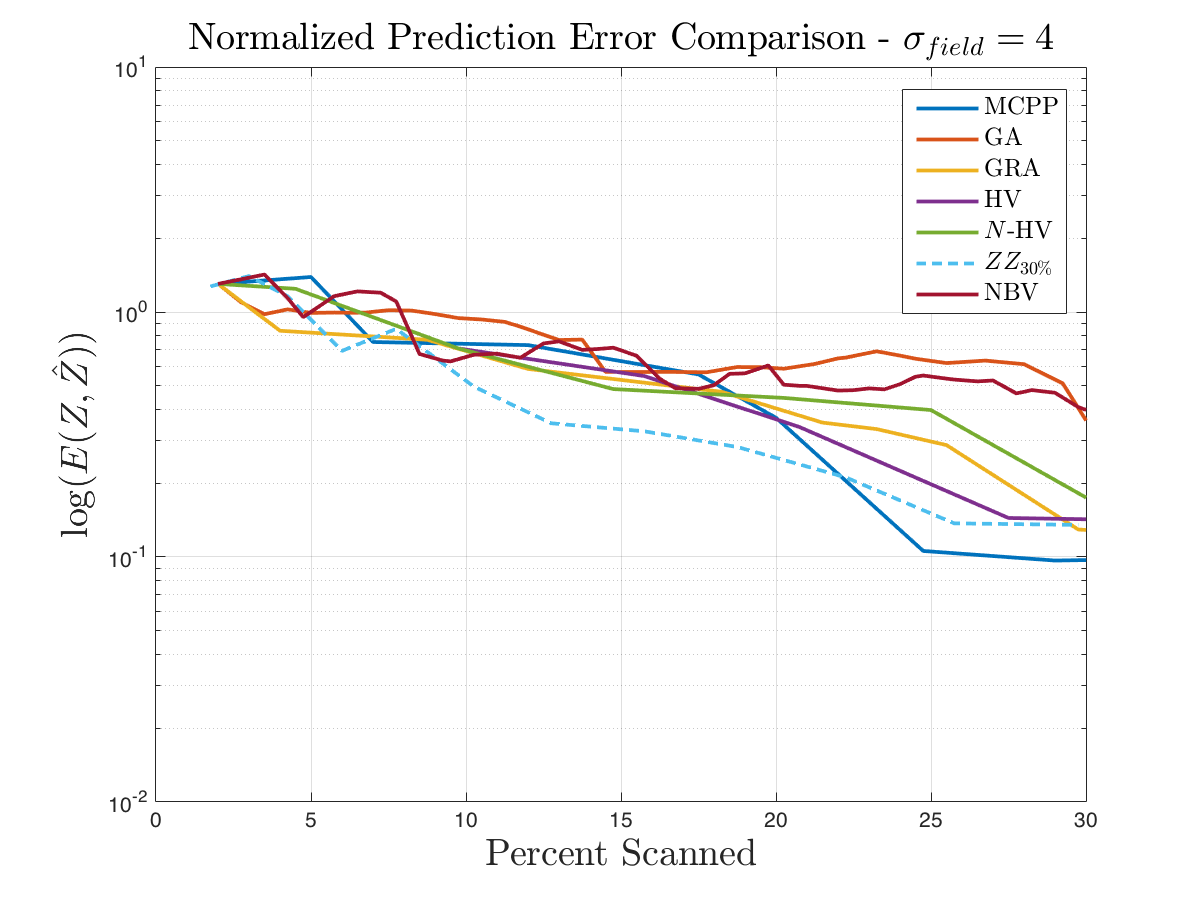
\includegraphics[width=\linewidth]{figures/results/normalized_errors_40p_20x20_sf_4_seed_2_app_10.png}
        \ssp
        \captionsetup{skip=0.20\baselineskip,size=footnotesize}
        \caption{Normalized prediction errors for each method.}
    \end{subfigure}%
    \begin{subfigure}[t]{0.5\textwidth}
        \centering
        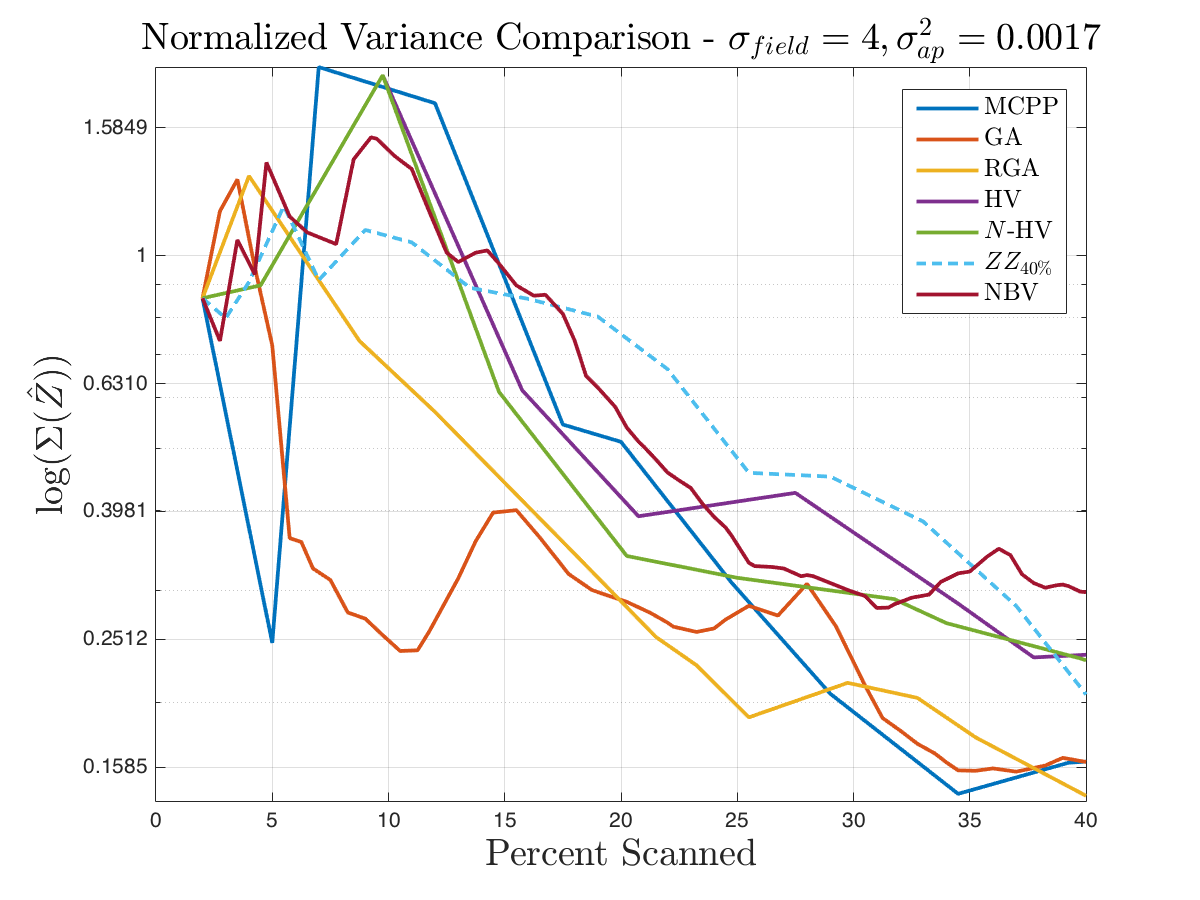
\includegraphics[width=\linewidth]{figures/results/normalized_variances_40p_20x20_sf_4_seed_2_app_10.png}
        \ssp
        \captionsetup{skip=0.20\baselineskip,size=footnotesize}
        \caption{Normalized prediction variances for each method.}
    \end{subfigure}%
    \ssp
    \captionsetup{skip=0.20\baselineskip}
    \caption{Prediction error and variances for an exploration of a field of size $20 \times 20$, $\sigma_{field} = 4$, random seed 2.}
    \label{fig:nbvcomp}
\end{figure}

\begin{figure}[htb!]
    \centering
    \begin{subfigure}[t]{0.3333\textwidth}
        \centering
        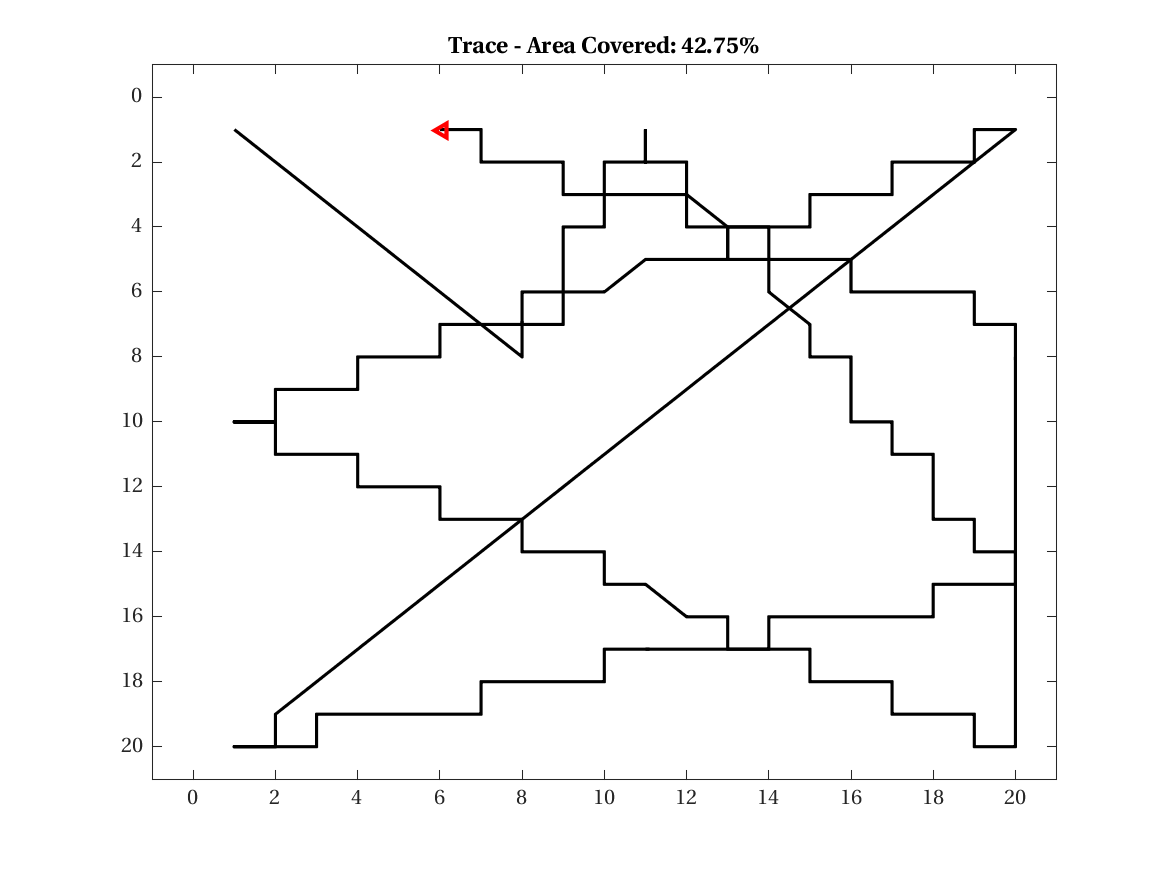
\includegraphics[width=\linewidth]{figures/hbresults/path_nhv_40p_20x20_sf_4_seed_2.png}
        \ssp
        \captionsetup{skip=0.20\baselineskip,size=footnotesize}
        \caption{Highest Variance}
    \end{subfigure}%
    \begin{subfigure}[t]{0.3333\textwidth}
        \centering
        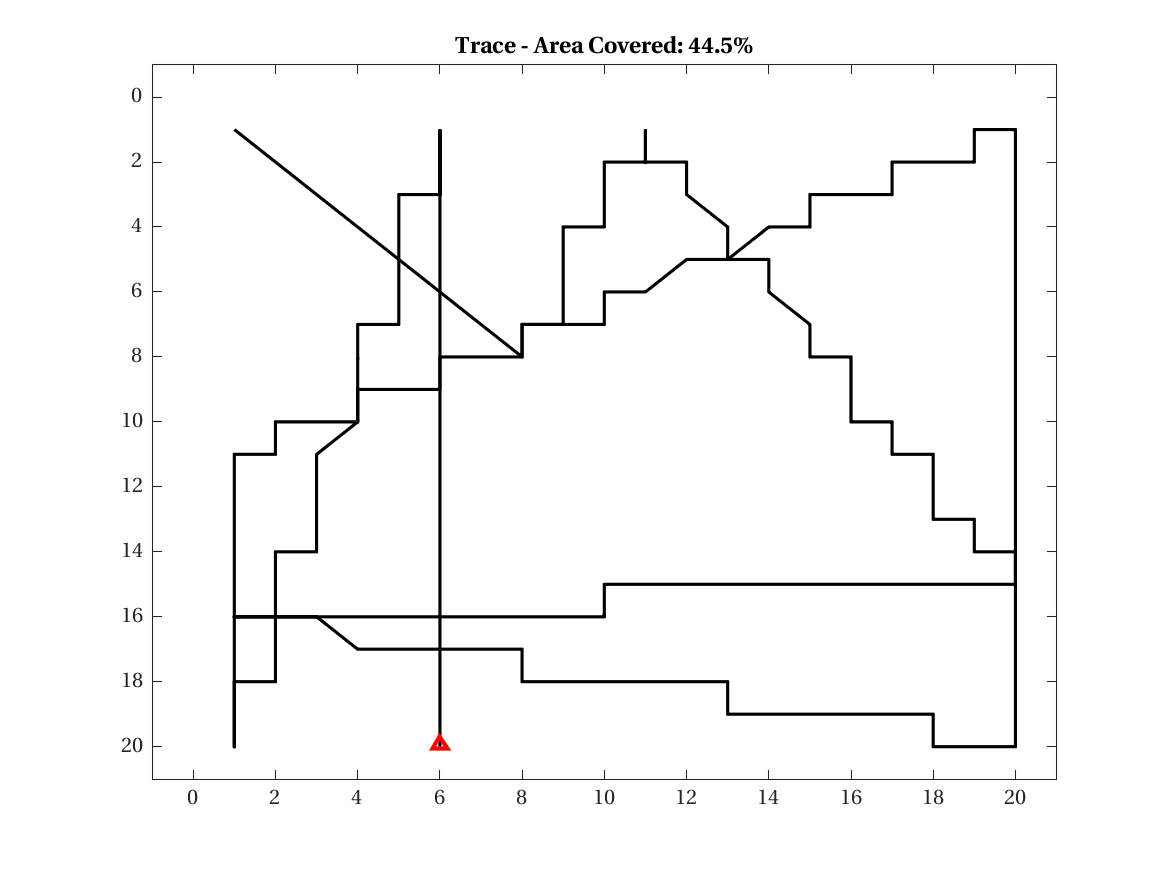
\includegraphics[width=\linewidth]{figures/hbresults/path_nnhv_40p_20x20_sf_4_seed_2.png}
        \ssp
        \captionsetup{skip=0.20\baselineskip,size=footnotesize}
        \caption{$N$ Highest Variance}
    \end{subfigure}%
    \begin{subfigure}[t]{0.3333\textwidth}
        \centering
        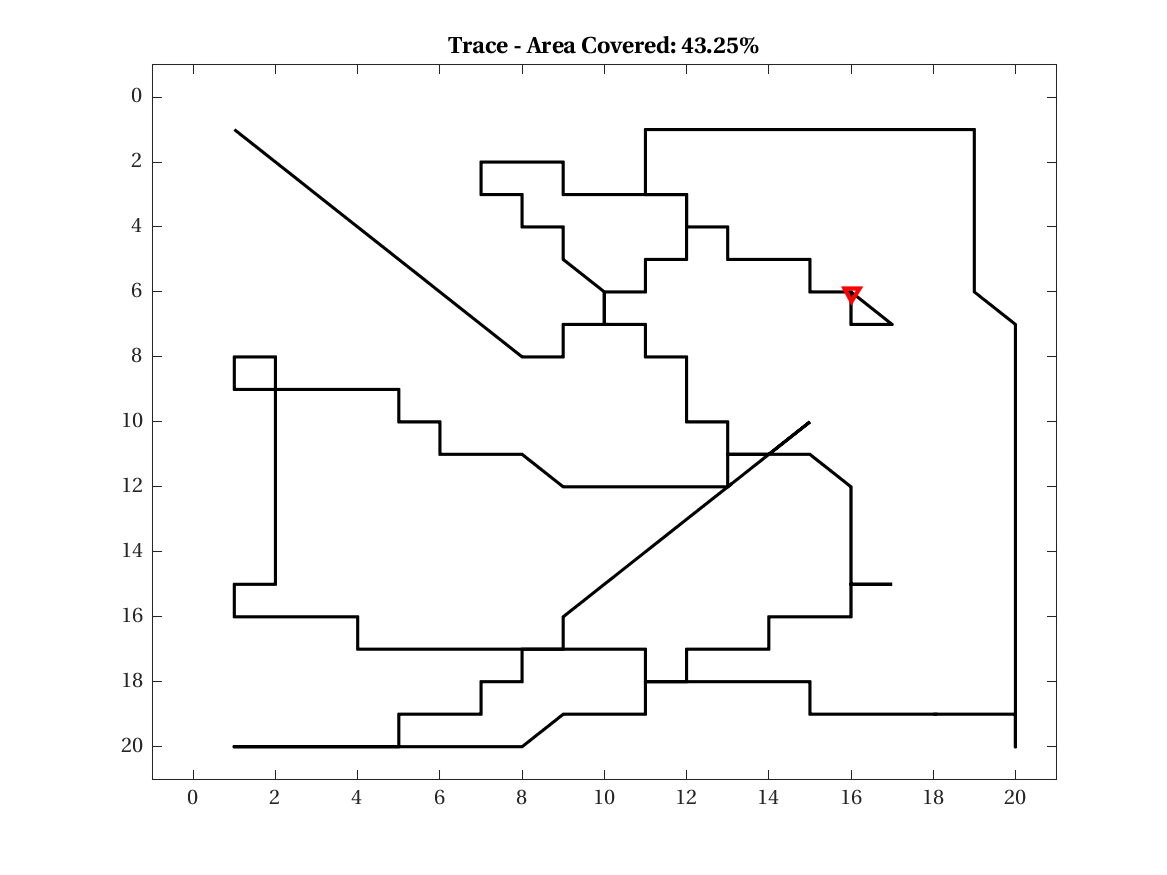
\includegraphics[width=\linewidth]{figures/hbresults/path_mc_40p_20x20_sf_4_seed_2.png}
        \ssp
        \captionsetup{skip=0.20\baselineskip,size=footnotesize}
        \caption{Monte Carlo}
    \end{subfigure}%
    \\
    \begin{subfigure}[t]{0.3333\textwidth}
        \centering
        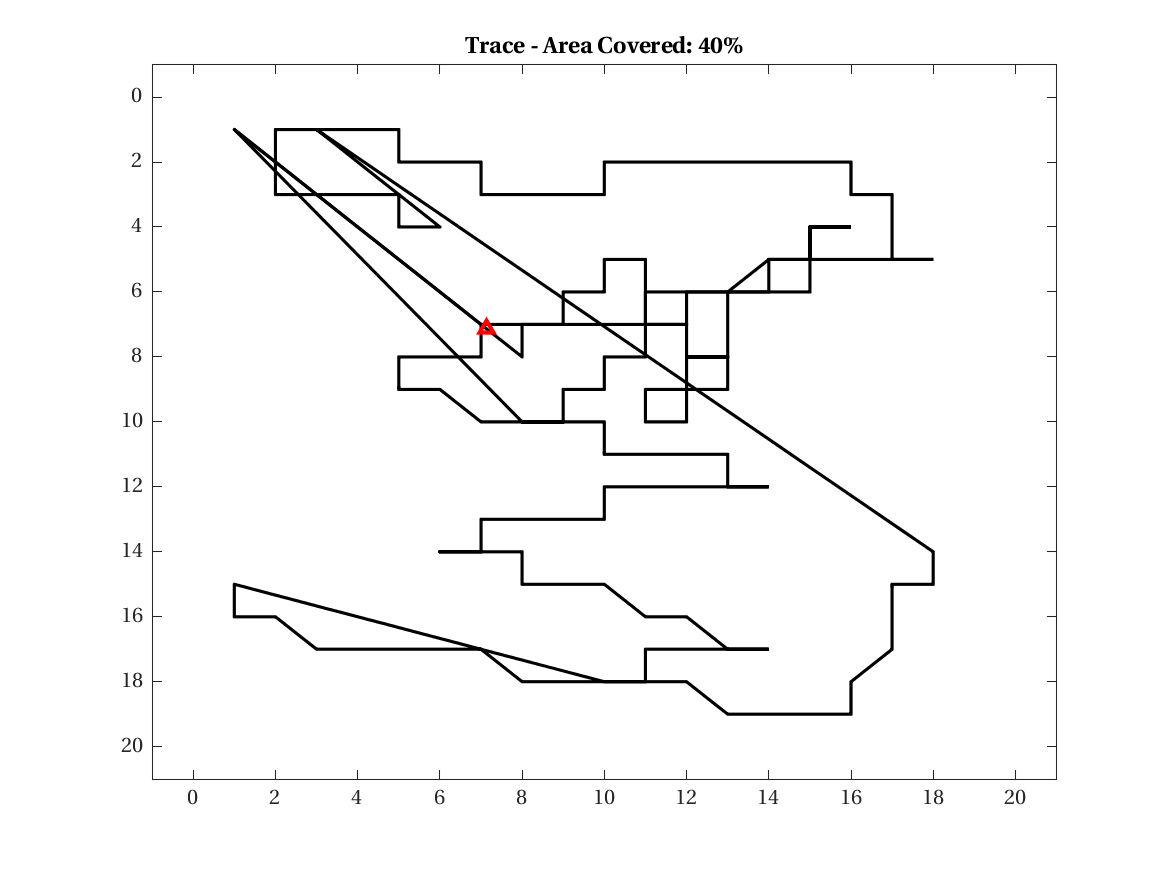
\includegraphics[width=\linewidth]{figures/hbresults/path_nbv_40p_20x20_sf_4_seed_2.png}
        \ssp
        \captionsetup{skip=0.20\baselineskip,size=footnotesize}
        \caption{Greedy NBV}
    \end{subfigure}%
    \begin{subfigure}[t]{0.3333\textwidth}
        \centering
        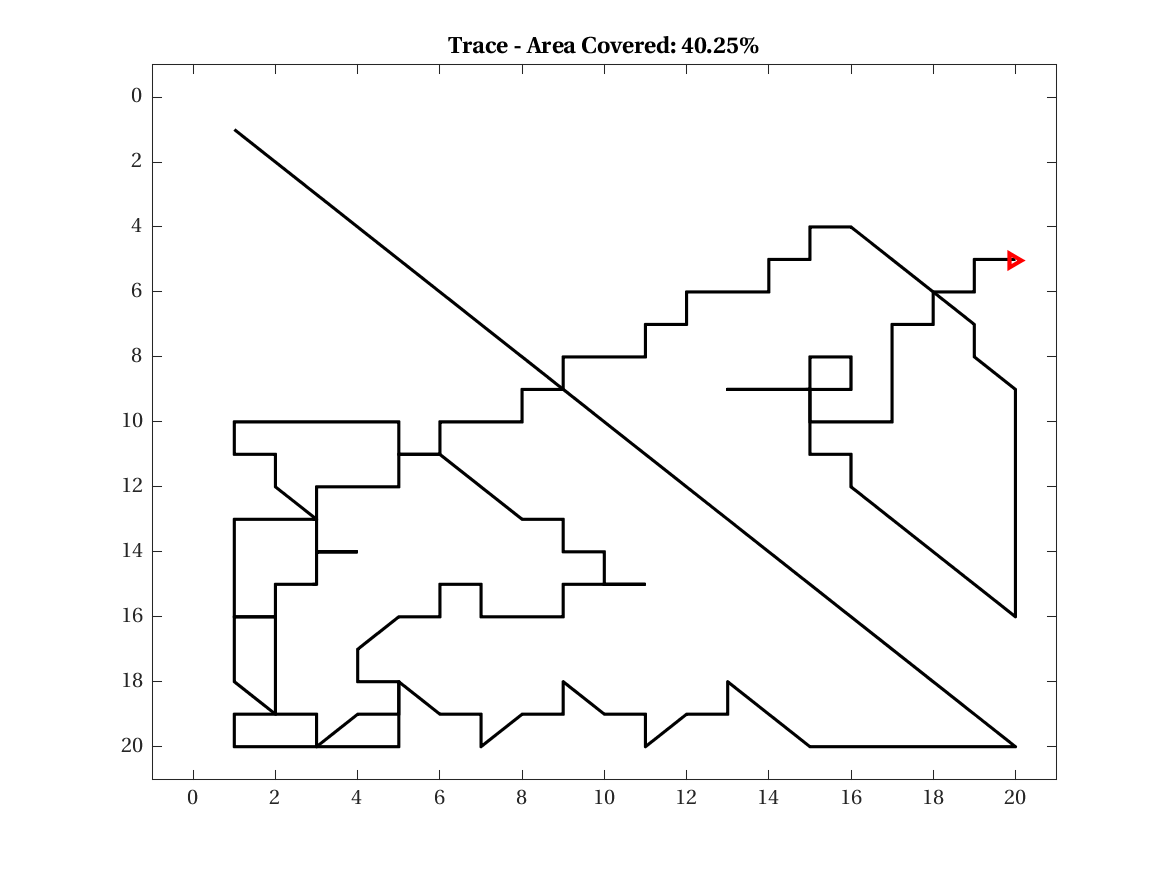
\includegraphics[width=\linewidth]{figures/hbresults/path_gradient_40p_20x20_sf_4_seed_2.png}
        \ssp
        \captionsetup{skip=0.20\baselineskip,size=footnotesize}
        \caption{Gradient Ascent}
    \end{subfigure}%
    \begin{subfigure}[t]{0.3333\textwidth}
        \centering
        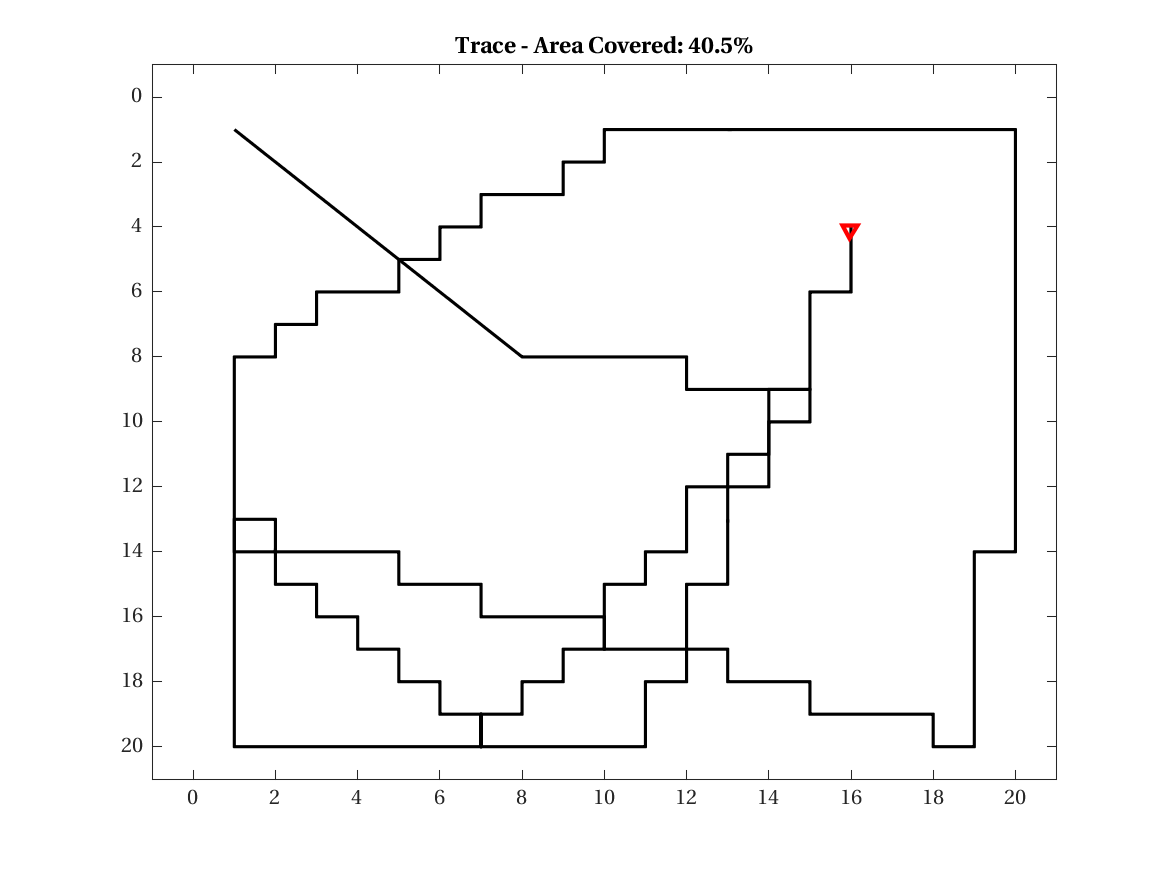
\includegraphics[width=\linewidth]{figures/hbresults/path_gr_40p_20x20_sf_4_seed_2.png}
        \ssp
        \captionsetup{skip=0.20\baselineskip,size=footnotesize}
        \caption{Range Gradient Ascent}
    \end{subfigure}%
    \\
    \begin{subfigure}[t]{0.3333\textwidth}
        \centering
        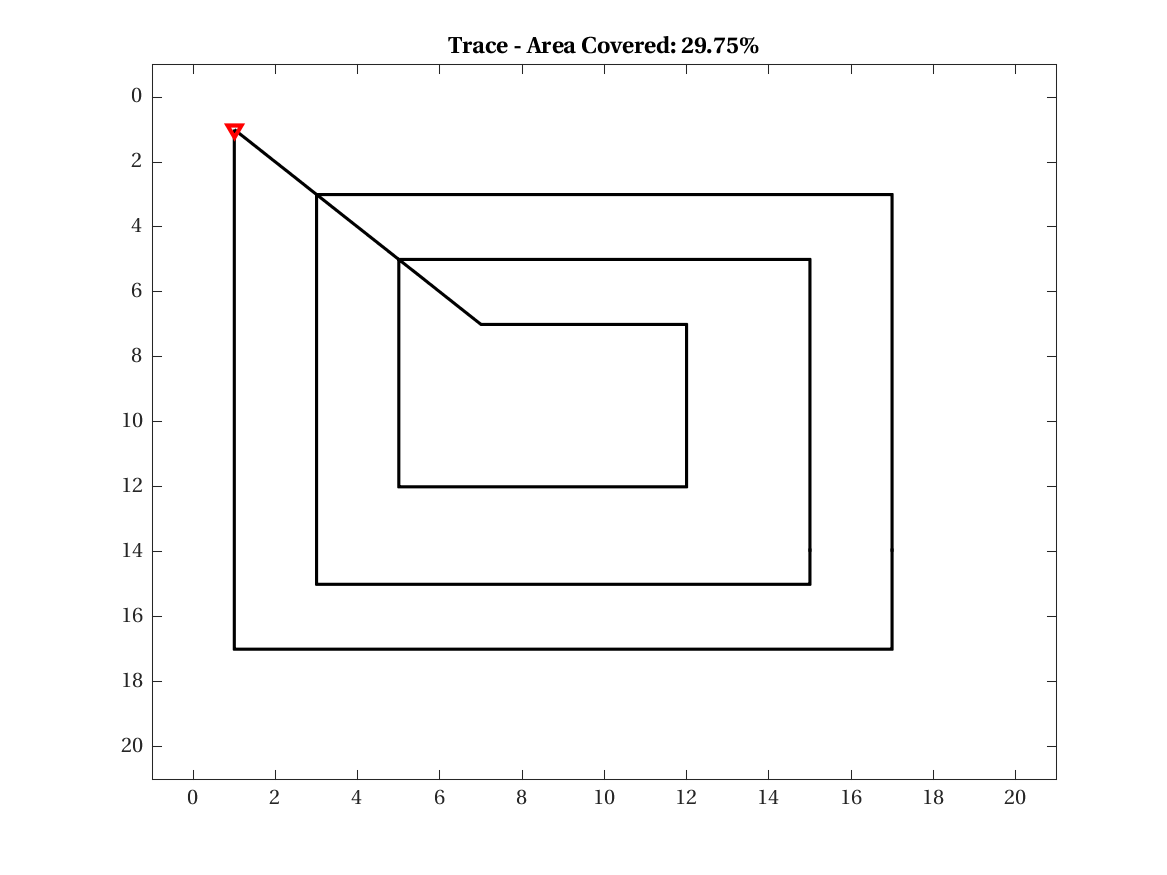
\includegraphics[width=\linewidth]{figures/hbresults/path_zz_40p_20x20_sf_4_seed_2.png}
        \ssp
        \captionsetup{skip=0.20\baselineskip,size=footnotesize}
        \caption{$ZZ_{40}$}
    \end{subfigure}%
    \ssp
    \captionsetup{skip=0.20\baselineskip}
    \caption{A $40\%$ scan limited exploration of a field of size $20 \times 20$, $\sigma_{field} = 4$, random seed 2.}
    \label{fig:nbvpathcomp}
\end{figure}

\FloatBarrier
\clearpage

\section{High Spatial Autocorrelation Results ($\sigma_{field} = 100$)} \label{sec:sigma100}
The methods will be compared on target fields generated with an autocorrelation factor, $\sigma_{field}$, equal to the field width. A Gaussian filter $G(x,y,100)$ (Equation \ref{eq:gauss_filt}), is convolved with all points on the field. Paths taken for each of the methods, except for the zig-zag method, are shown for scan areas nearest to the $10\%$, $20\%$, and $30\%$ marks in Figure \ref{fig:sf100}.\\\\

\begin{figure}[htb!]
    \centering
    \begin{subfigure}[t]{0.50\textwidth}
        \centering
        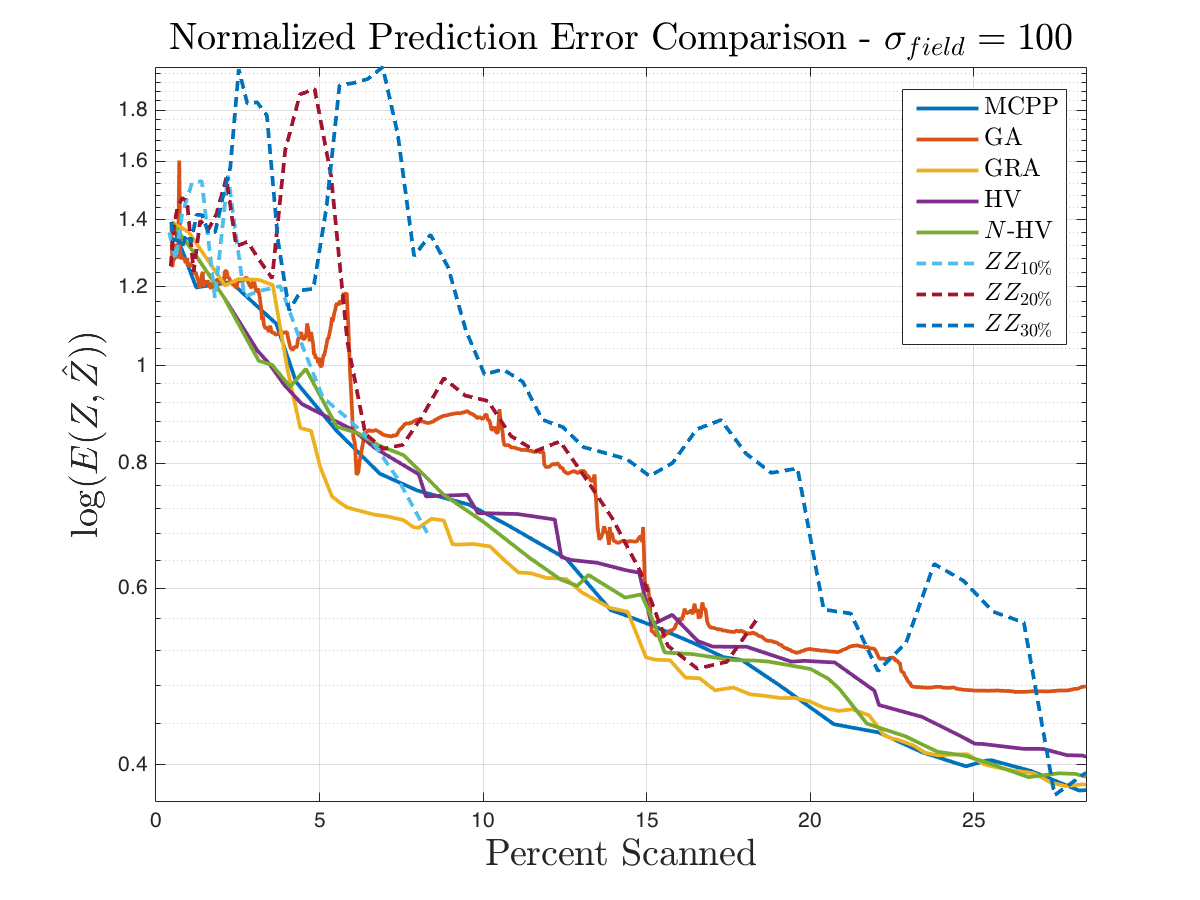
\includegraphics[width=\linewidth]{figures/results/normalized_errors_30p_100x100_sf_100_seed_2_app_50.png}
        \ssp
        \captionsetup{skip=0.20\baselineskip,size=footnotesize}
        \caption{Normalized prediction errors for each method.}
    \end{subfigure}%
    \begin{subfigure}[t]{0.50\textwidth}
        \centering
        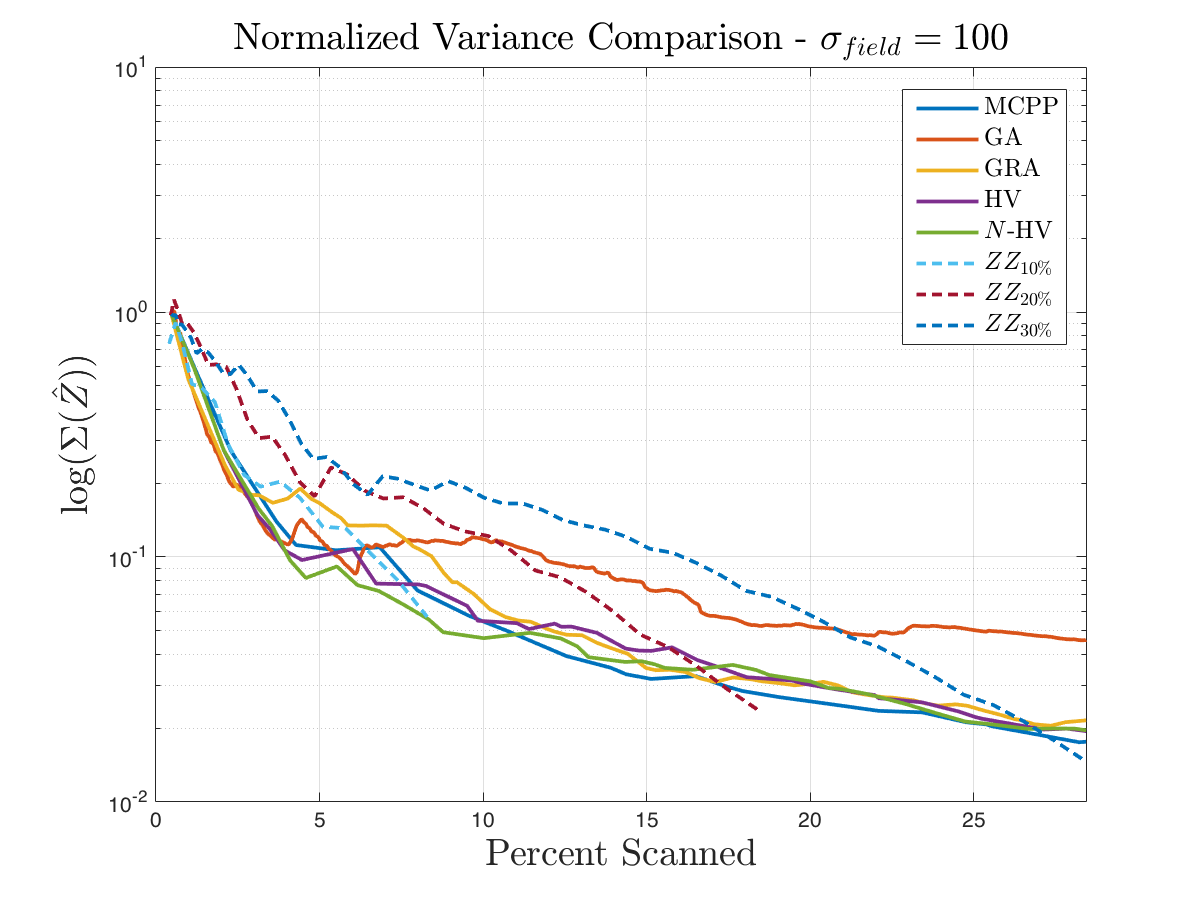
\includegraphics[width=\linewidth]{figures/results/normalized_variances_30p_100x100_sf_100_seed_2_app_50.png}
        \ssp
        \captionsetup{skip=0.20\baselineskip,size=footnotesize}
        \caption{Normalized prediction variances for each method.}
    \end{subfigure}%
    \ssp
    \captionsetup{skip=0.20\baselineskip}
    \caption{Prediction error and variances for an exploration of a field of size $100 \times 100$, $\sigma_{field} = 100$, random seed 2.}
    \label{fig:errvar100}
\end{figure}

\begin{figure}[htb!]
    \centering
        \begin{subfigure}[t]{0.32\textwidth}
        \centering
        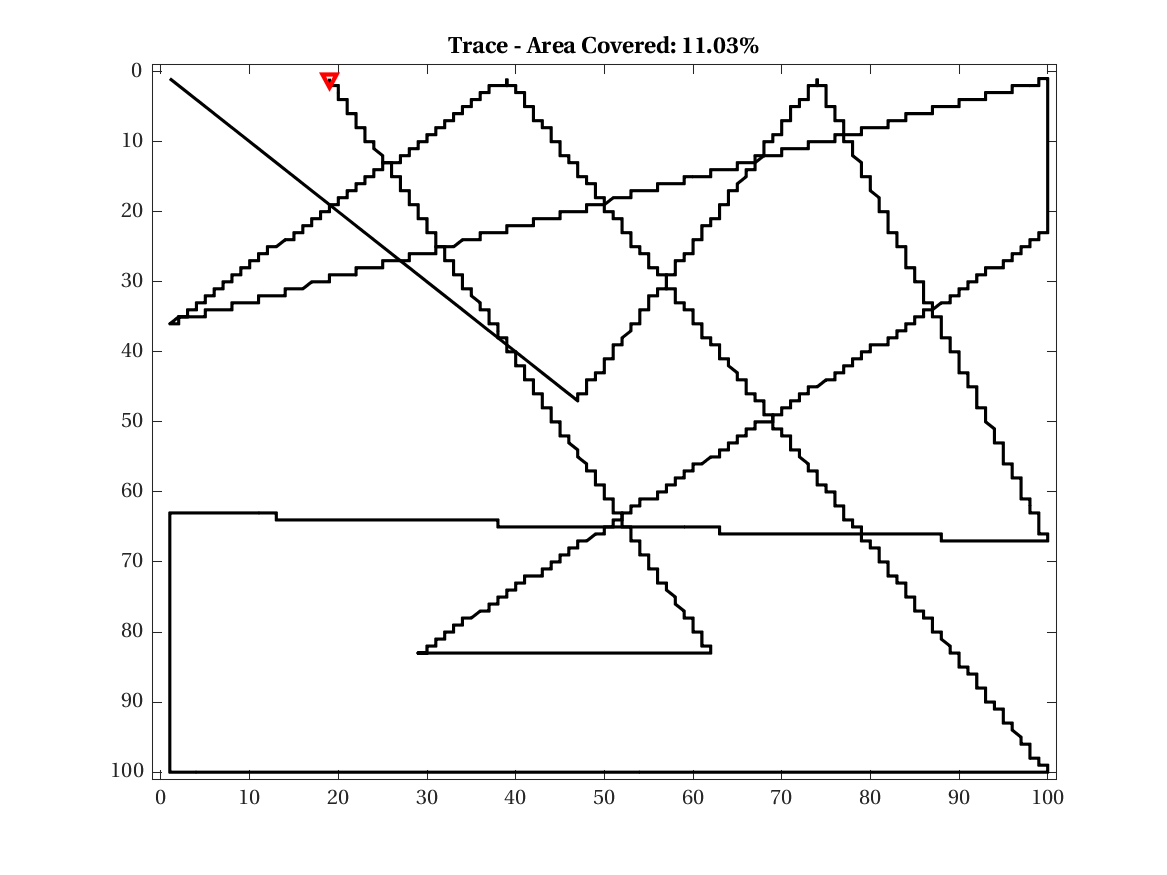
\includegraphics[width=\linewidth]{figures/hbresults/path_nhv_10p_100x100_sf_100_seed_2.png}
        \ssp
        \captionsetup{skip=0.20\baselineskip,size=footnotesize}
        \caption{Highest Variance ($10\%$)}
    \end{subfigure}%
    \begin{subfigure}[t]{0.32\textwidth}
        \centering
        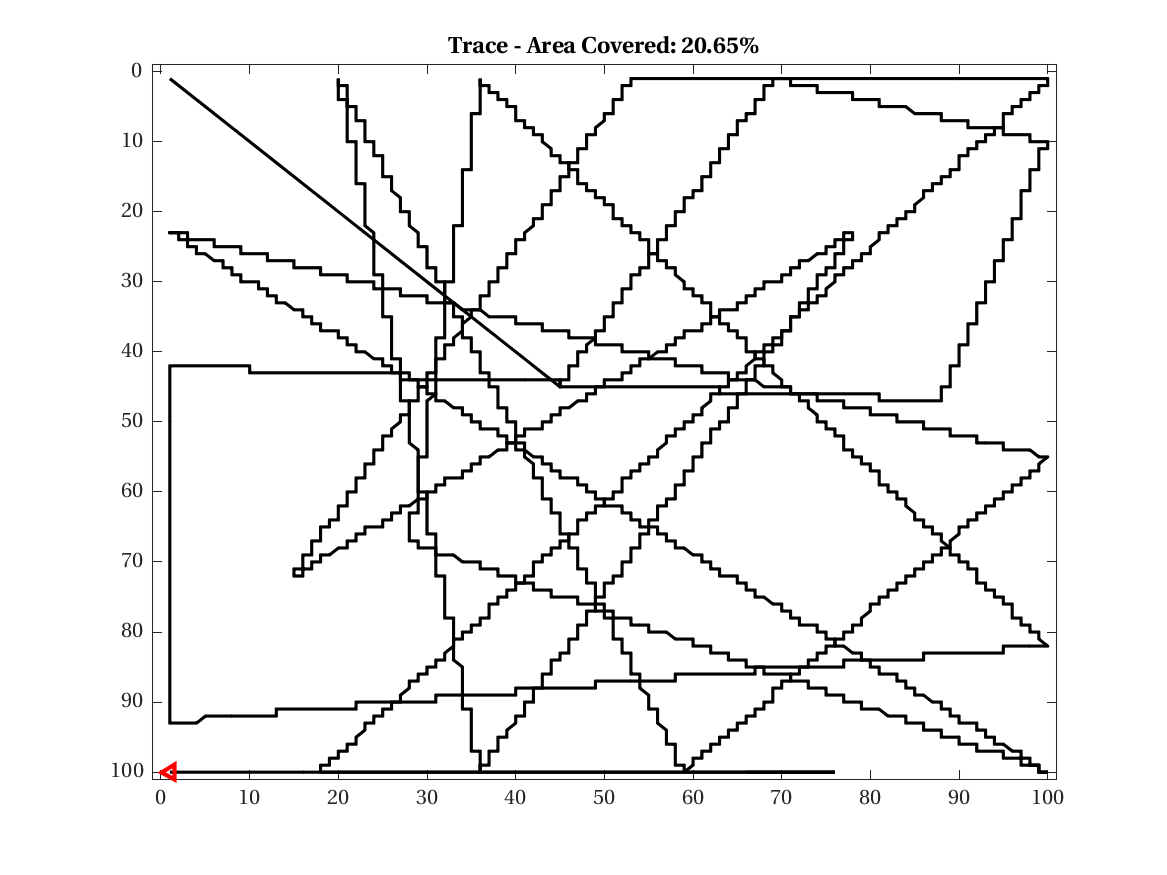
\includegraphics[width=\linewidth]{figures/hbresults/path_nhv_20p_100x100_sf_100_seed_2.png}
        \ssp
        \captionsetup{skip=0.20\baselineskip,size=footnotesize}
        \caption{Highest Variance ($20\%$)}
    \end{subfigure}%
    \begin{subfigure}[t]{0.32\textwidth}
        \centering
        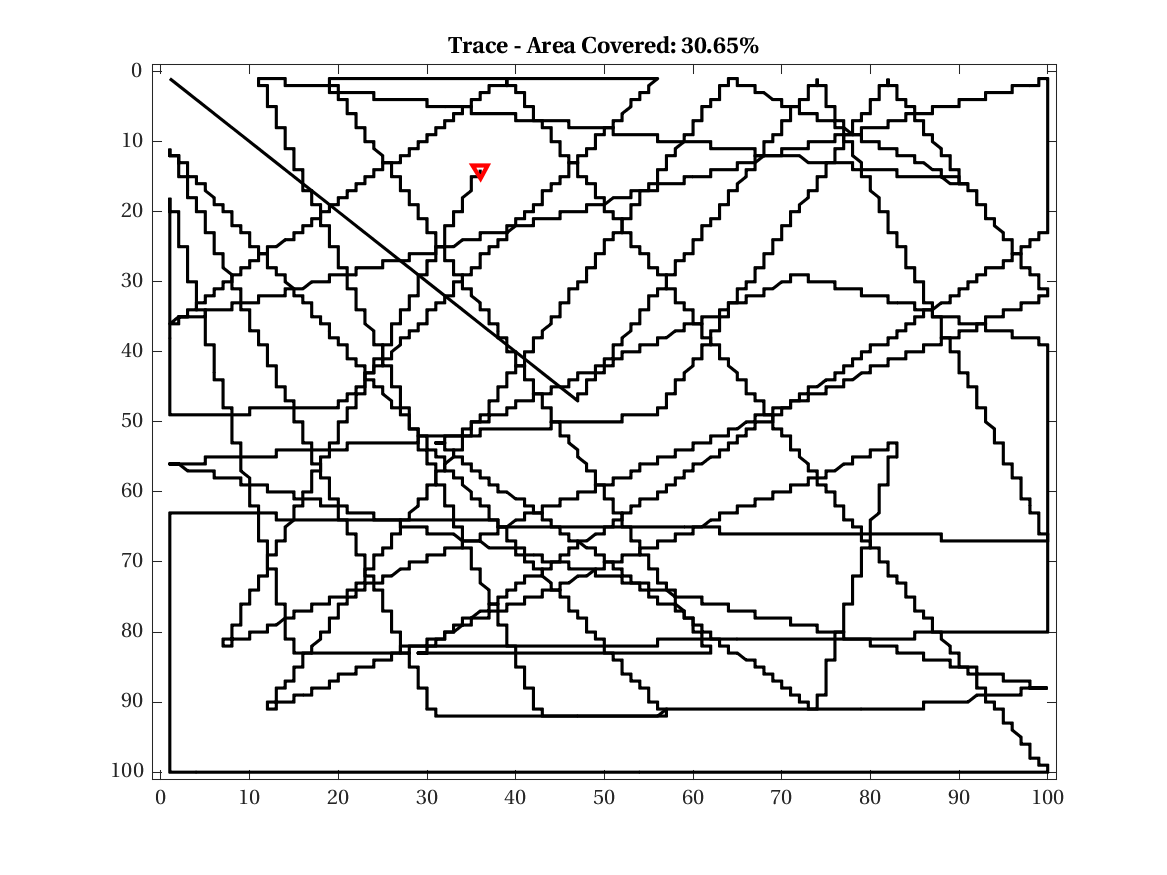
\includegraphics[width=\linewidth]{figures/hbresults/path_nhv_30p_100x100_sf_100_seed_2.png}
        \ssp
        \captionsetup{skip=0.20\baselineskip,size=footnotesize}
        \caption{Highest Variance ($30\%$)}
    \end{subfigure}%
    \\
    \begin{subfigure}[t]{0.32\textwidth}
        \centering
        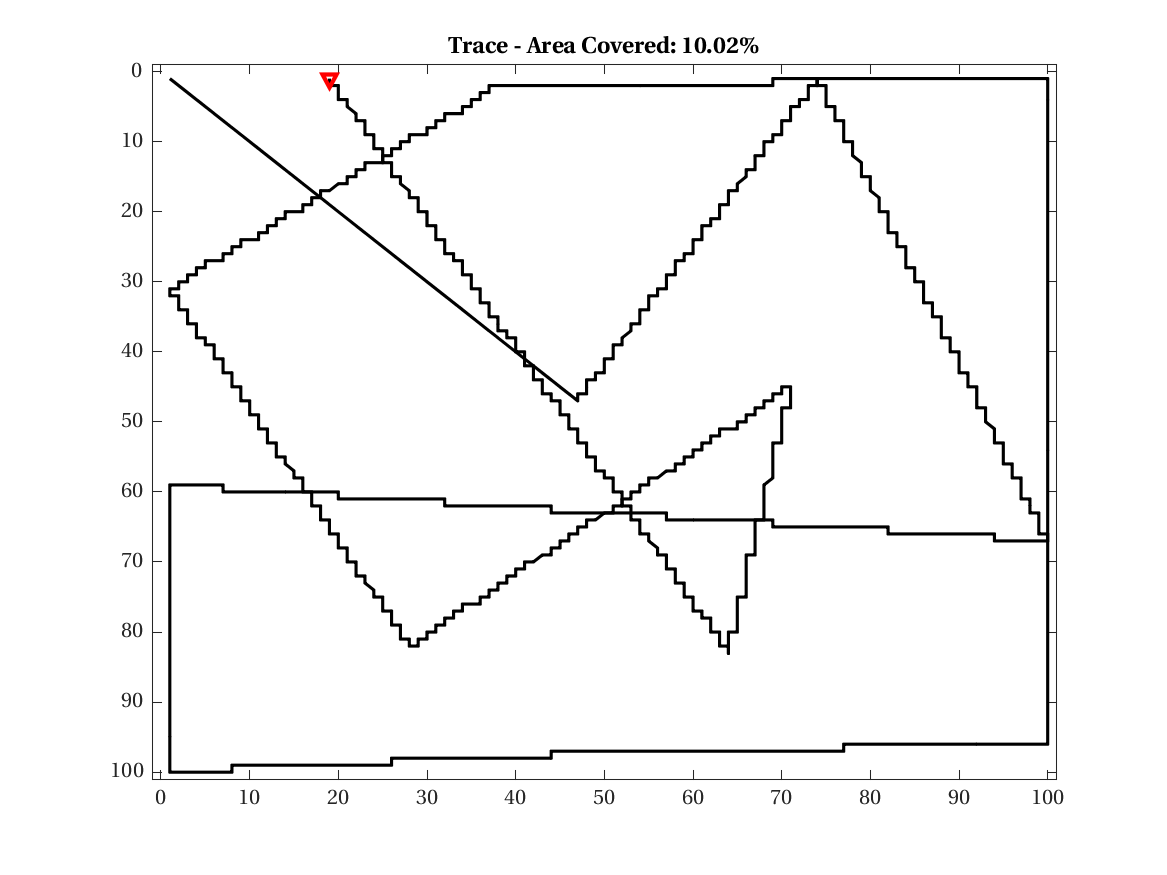
\includegraphics[width=\linewidth]{figures/hbresults/path_nnhv_10p_100x100_sf_100_seed_2.png}
        \ssp
        \captionsetup{skip=0.20\baselineskip,size=footnotesize}
        \caption{$N$ Highest Variance ($10\%$)}
    \end{subfigure}%
    \begin{subfigure}[t]{0.32\textwidth}
        \centering
        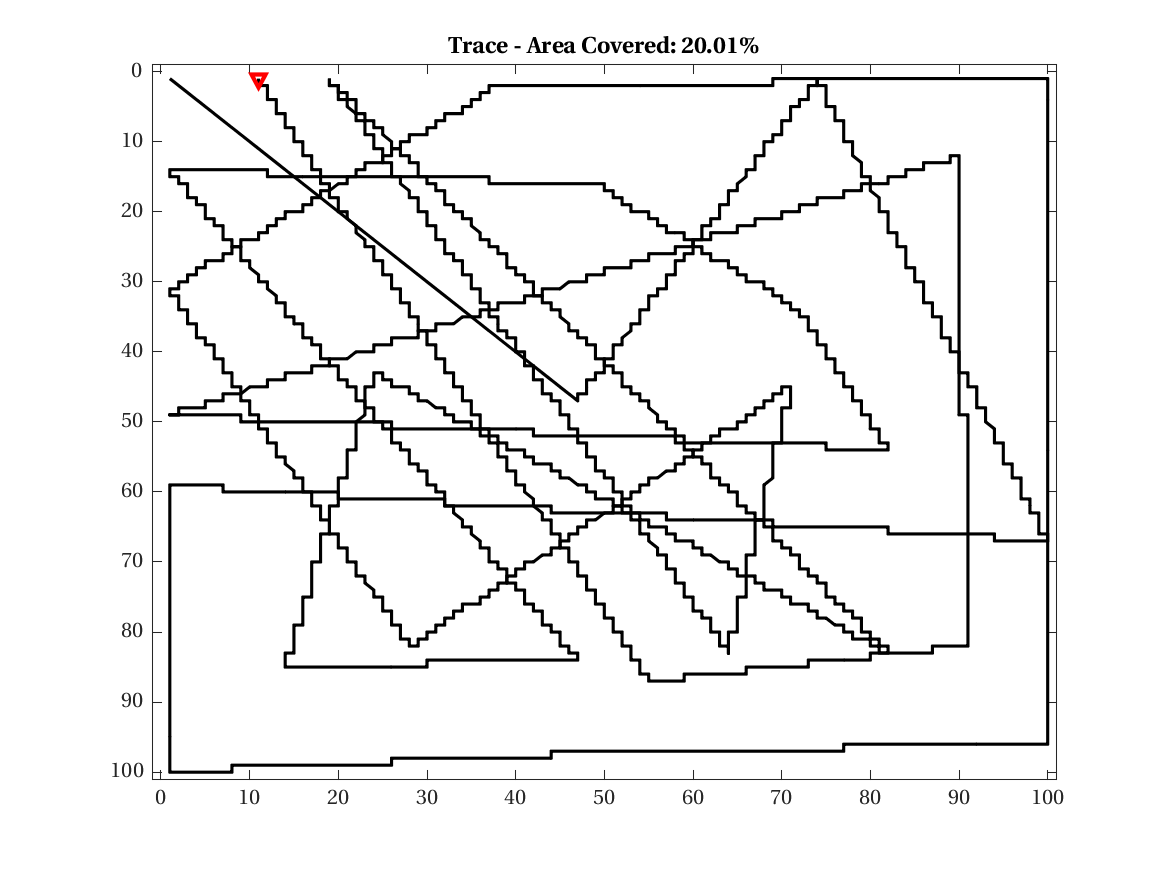
\includegraphics[width=\linewidth]{figures/hbresults/path_nnhv_20p_100x100_sf_100_seed_2.png}
        \ssp
        \captionsetup{skip=0.20\baselineskip,size=footnotesize}
        \caption{$N$ Highest Variance ($20\%$)}
    \end{subfigure}%
    \begin{subfigure}[t]{0.32\textwidth}
        \centering
        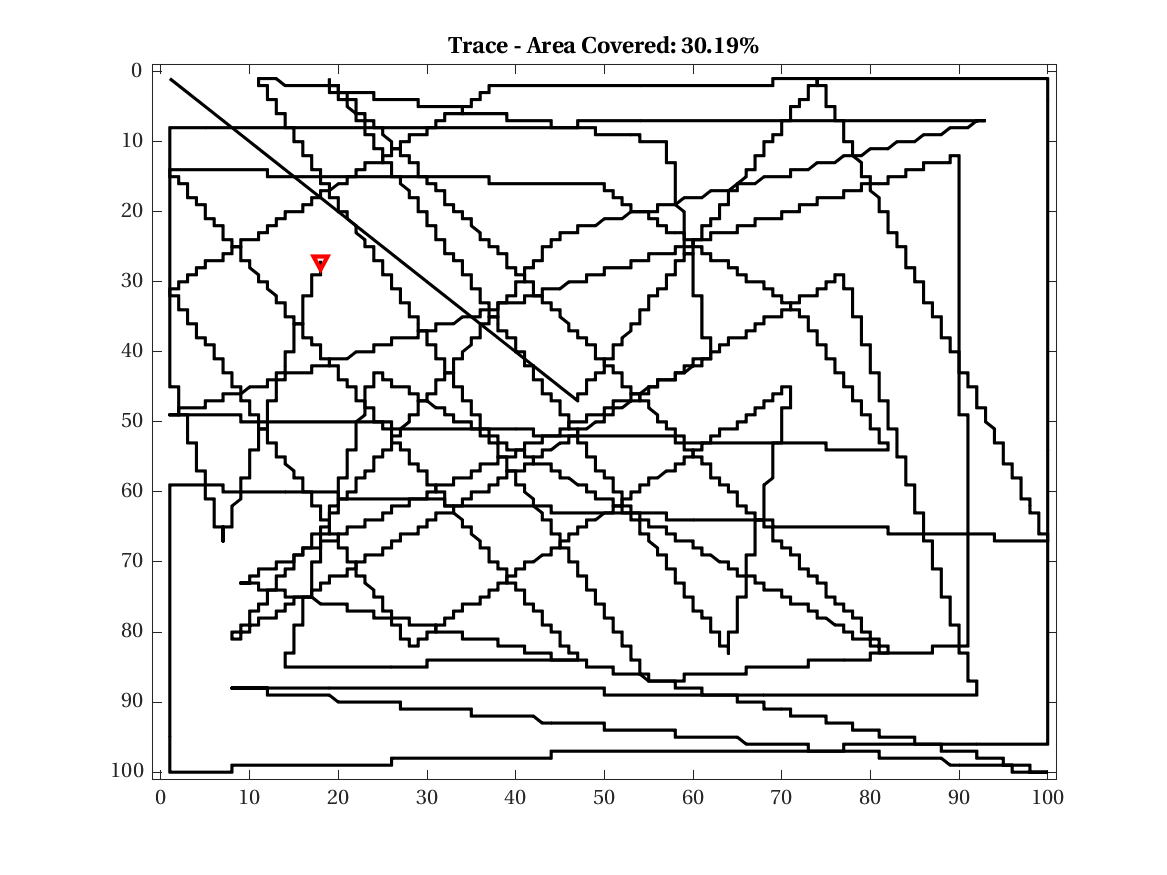
\includegraphics[width=\linewidth]{figures/hbresults/path_nnhv_30p_100x100_sf_100_seed_2.png}
        \ssp
        \captionsetup{skip=0.20\baselineskip,size=footnotesize}
        \caption{$N$ Highest Variance ($30\%$)}
    \end{subfigure}%
    \\
    \begin{subfigure}[t]{0.32\textwidth}
        \centering
        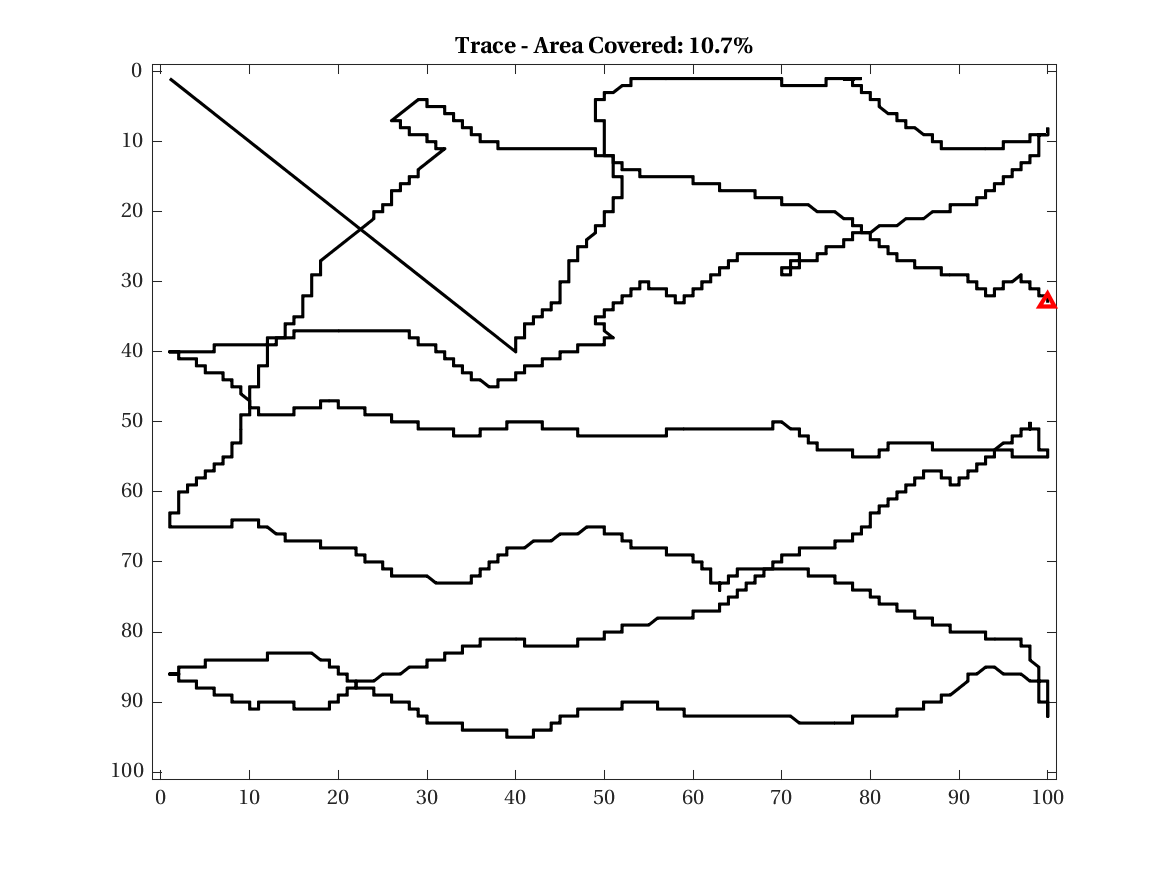
\includegraphics[width=\linewidth]{figures/hbresults/path_mc_10p_100x100_sf_100_seed_2.png}
        \ssp
        \captionsetup{skip=0.20\baselineskip,size=footnotesize}
        \caption{Monte Carlo ($10\%$)}
    \end{subfigure}%
    \begin{subfigure}[t]{0.32\textwidth}
        \centering
        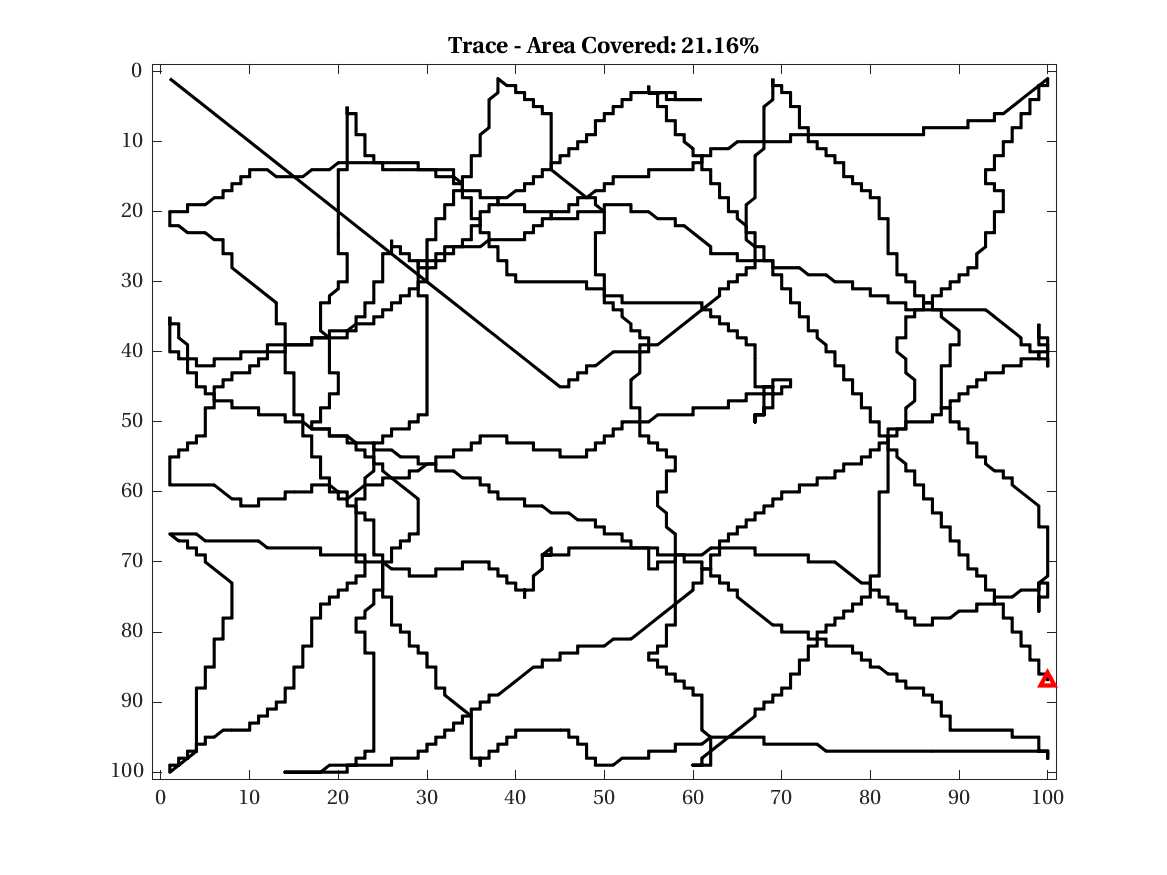
\includegraphics[width=\linewidth]{figures/hbresults/path_mc_20p_100x100_sf_100_seed_2.png}
        \ssp
        \captionsetup{skip=0.20\baselineskip,size=footnotesize}
        \caption{Monte Carlo ($20\%$)}
    \end{subfigure}%
    \begin{subfigure}[t]{0.32\textwidth}
        \centering
        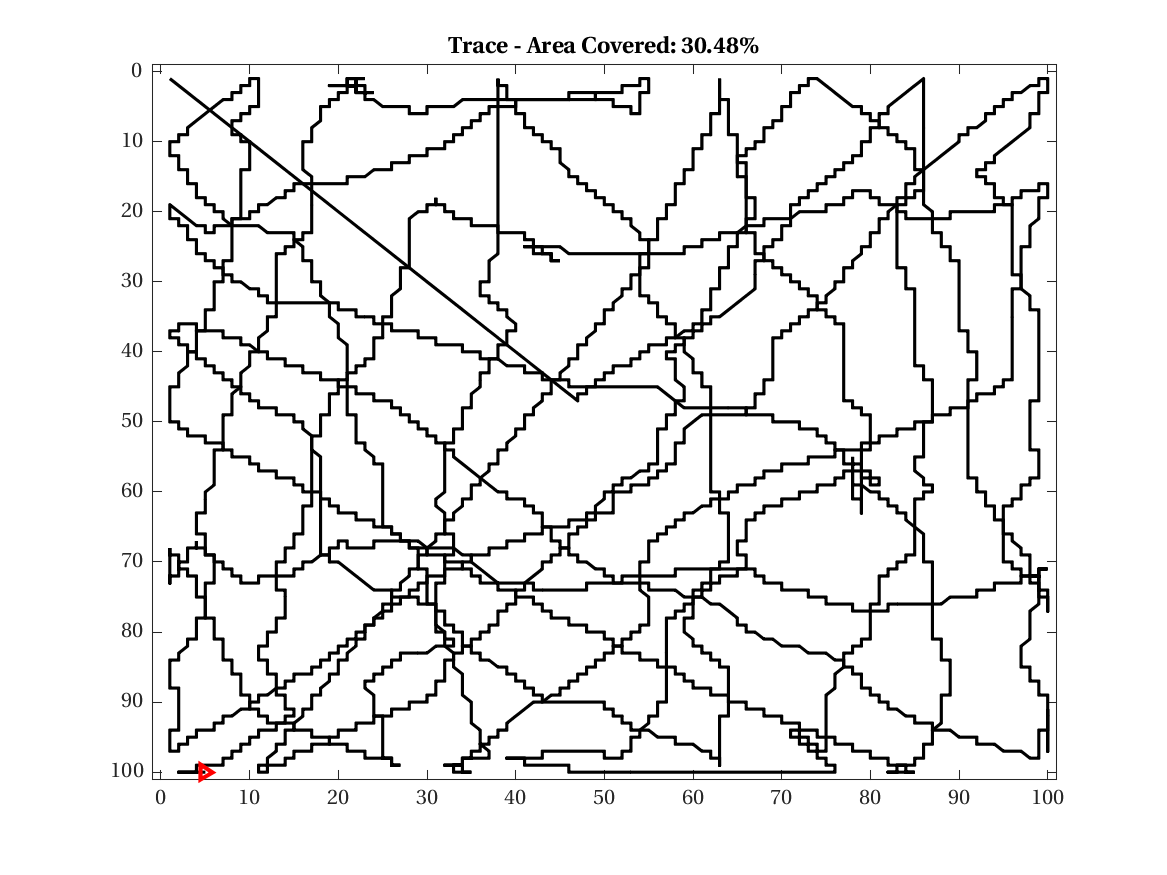
\includegraphics[width=\linewidth]{figures/hbresults/path_mc_30p_100x100_sf_100_seed_2.png}
        \ssp
        \captionsetup{skip=0.20\baselineskip,size=footnotesize}
        \caption{Monte Carlo ($30\%$)}
    \end{subfigure}%
    \\
    \begin{subfigure}[t]{0.32\textwidth}
        \centering
        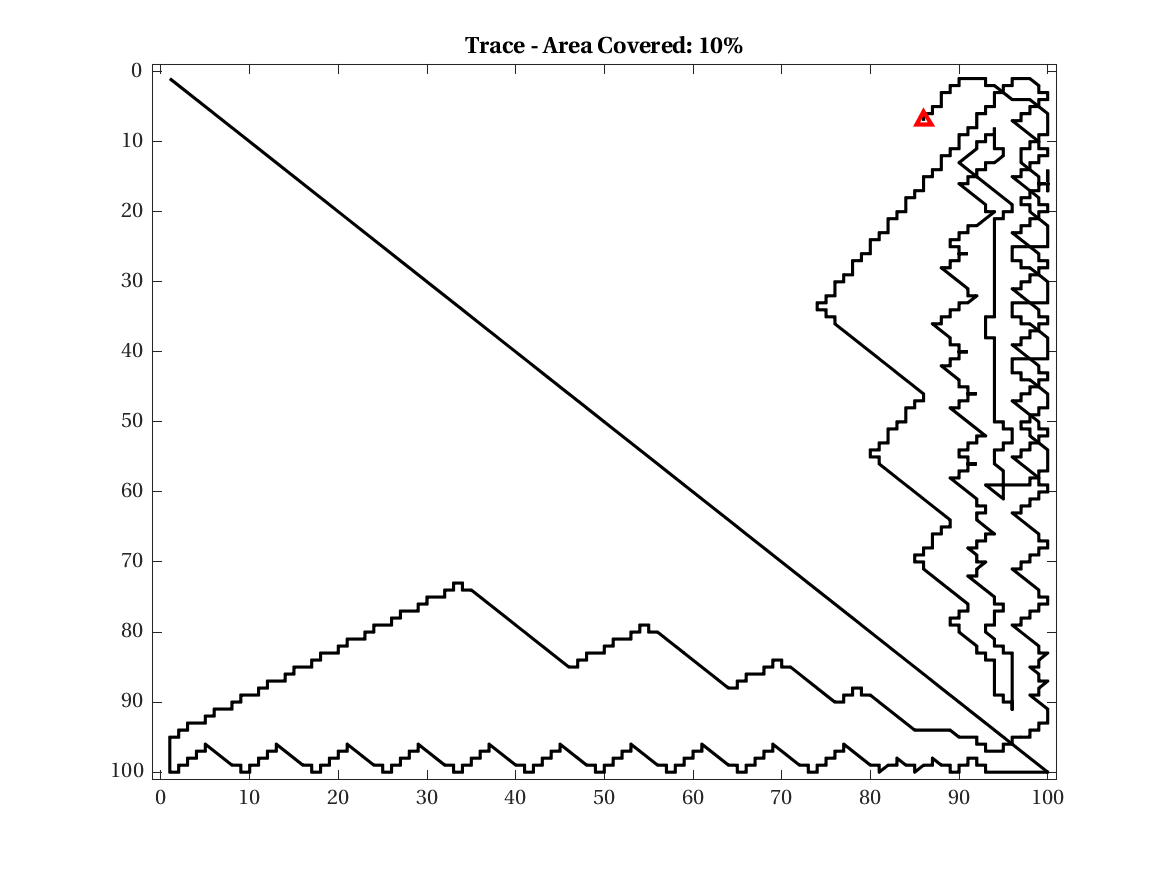
\includegraphics[width=\linewidth]{figures/hbresults/path_gradient_10p_100x100_sf_100_seed_2.png}
        \ssp
        \captionsetup{skip=0.20\baselineskip,size=footnotesize}
        \caption{Gradient Ascent ($10\%$)}
    \end{subfigure}%
    \begin{subfigure}[t]{0.32\textwidth}
        \centering
        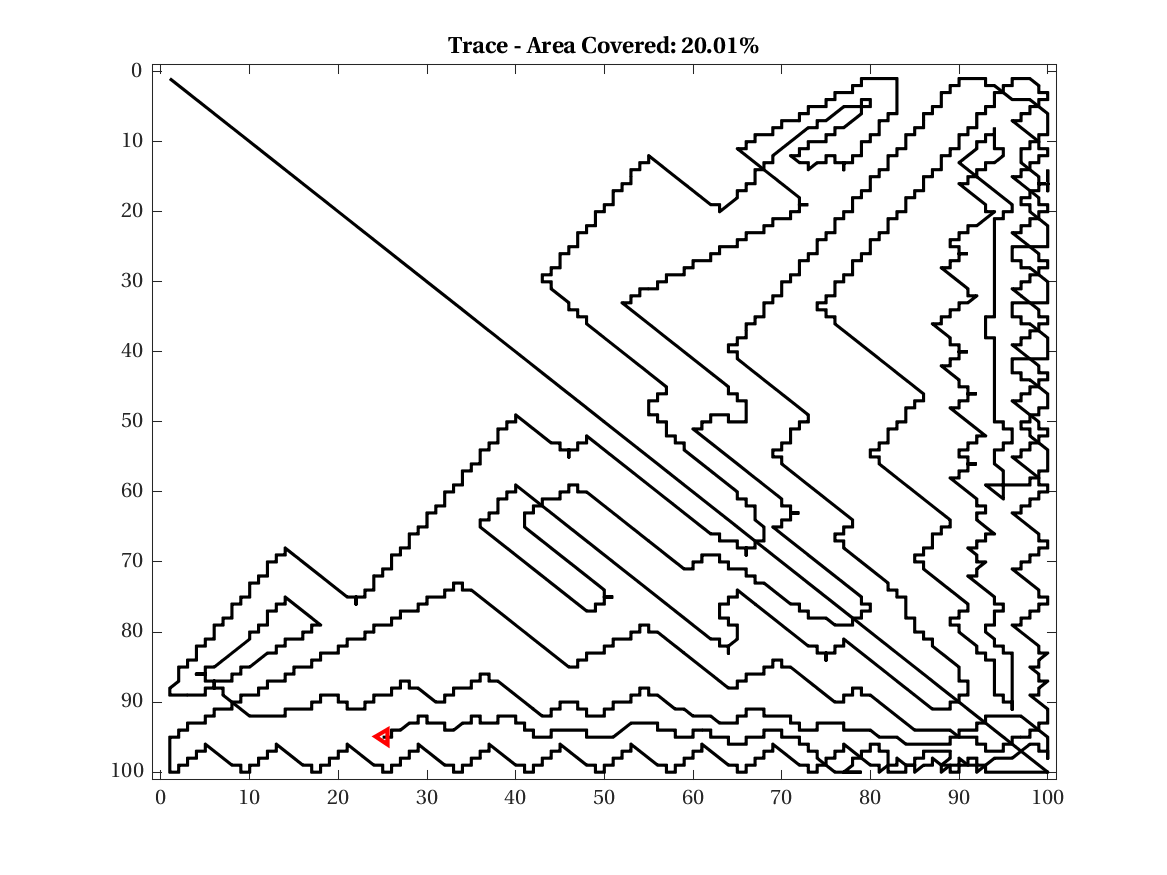
\includegraphics[width=\linewidth]{figures/hbresults/path_gradient_20p_100x100_sf_100_seed_2.png}
        \ssp
        \captionsetup{skip=0.20\baselineskip,size=footnotesize}
        \caption{Gradient Ascent ($20\%$)}
    \end{subfigure}%
    \begin{subfigure}[t]{0.32\textwidth}
        \centering
        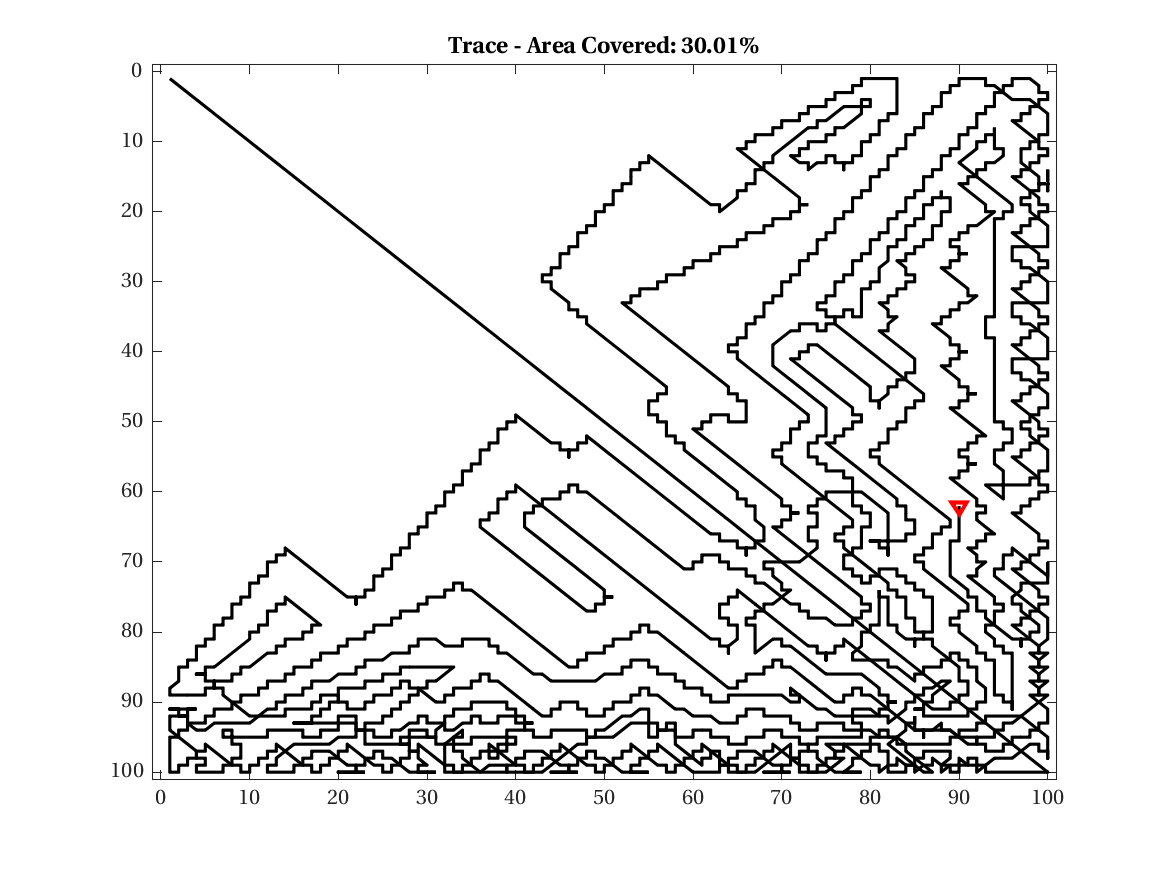
\includegraphics[width=\linewidth]{figures/hbresults/path_gradient_30p_100x100_sf_100_seed_2.png}
        \ssp
        \captionsetup{skip=0.20\baselineskip,size=footnotesize}
        \caption{Gradient Ascent ($30\%$)}
    \end{subfigure}%
    \\
    \begin{subfigure}[t]{0.32\textwidth}
        \centering
        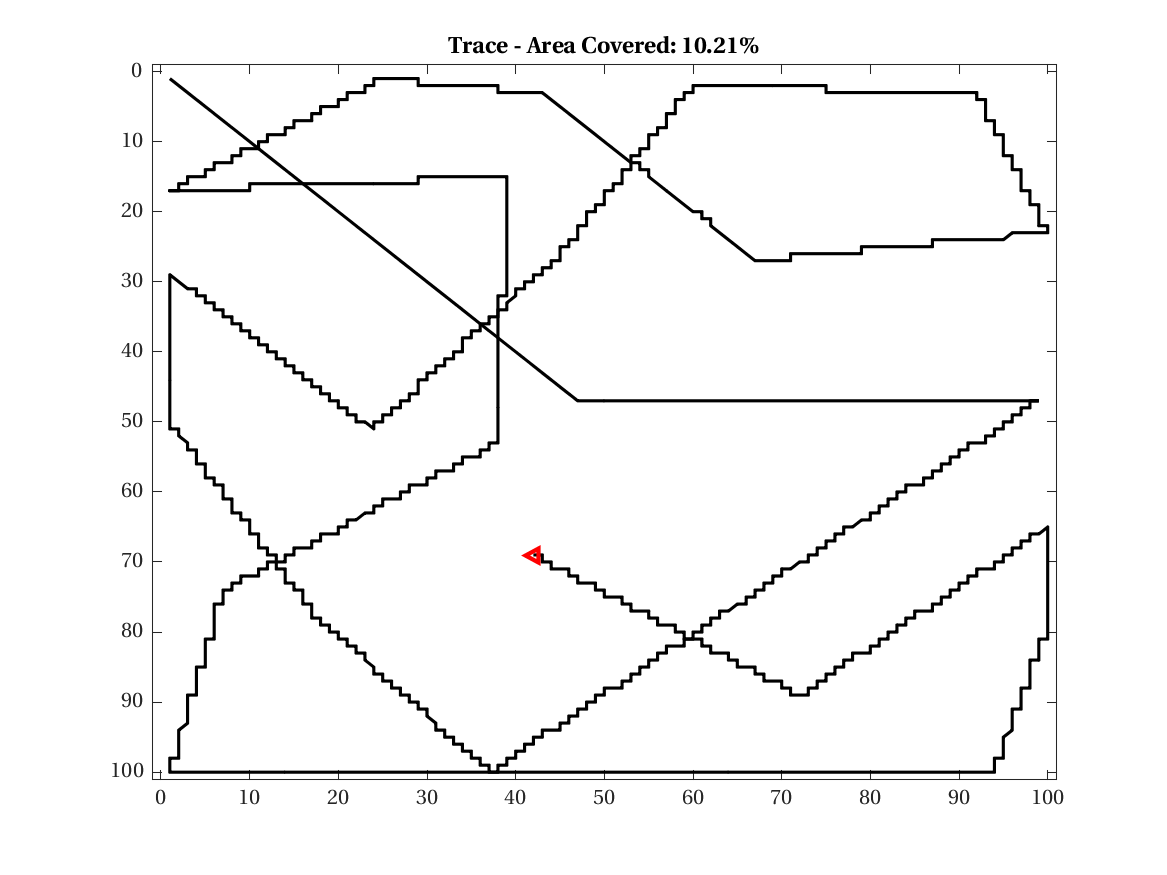
\includegraphics[width=\linewidth]{figures/hbresults/path_gr_10p_100x100_sf_100_seed_2.png}
        \ssp
        \captionsetup{skip=0.20\baselineskip,size=footnotesize}
        \caption{Range Gradient Ascent ($10\%$)}
    \end{subfigure}%
    \begin{subfigure}[t]{0.32\textwidth}
        \centering
        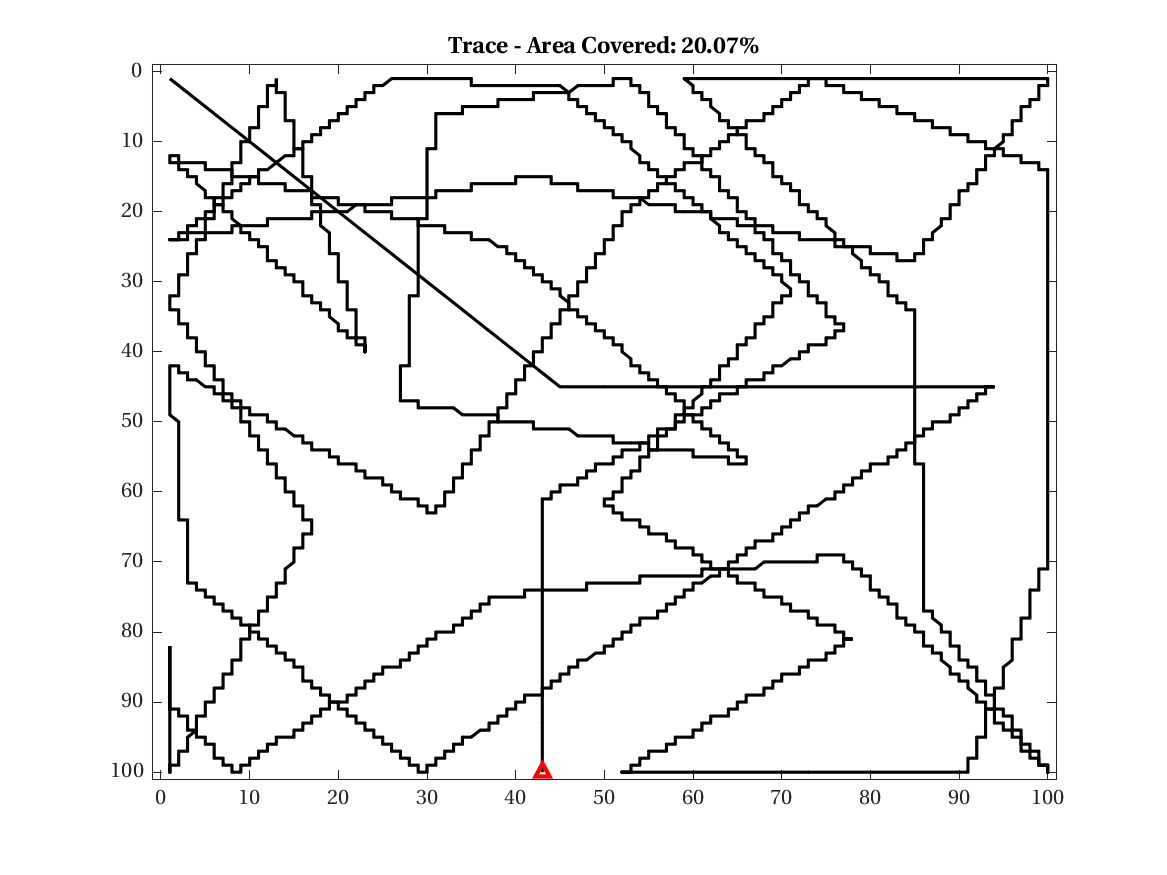
\includegraphics[width=\linewidth]{figures/hbresults/path_gr_20p_100x100_sf_100_seed_2.png}
        \ssp
        \captionsetup{skip=0.20\baselineskip,size=footnotesize}
        \caption{Range Gradient Ascent ($20\%$)}
    \end{subfigure}%
    \begin{subfigure}[t]{0.32\textwidth}
        \centering
        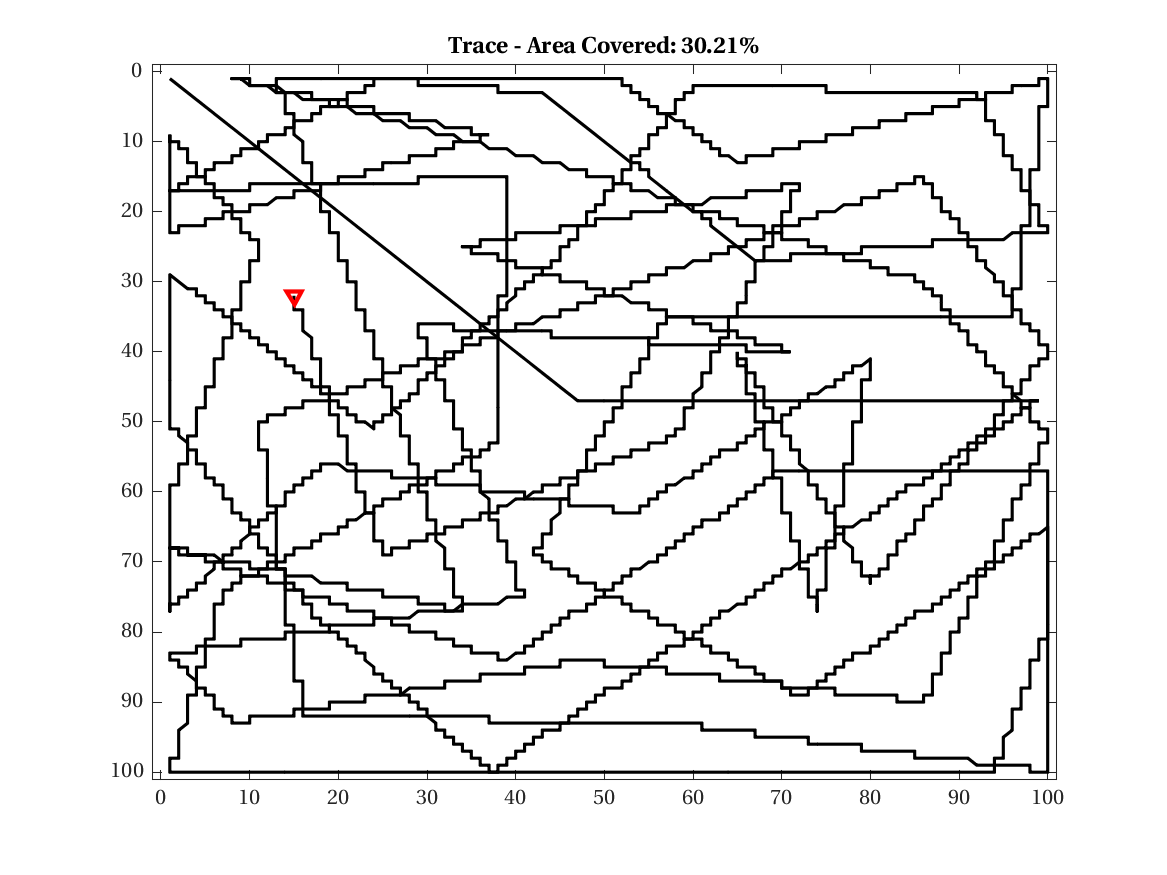
\includegraphics[width=\linewidth]{figures/hbresults/path_gr_30p_100x100_sf_100_seed_2.png}
        \ssp
        \captionsetup{skip=0.20\baselineskip,size=footnotesize}
        \caption{Range Gradient Ascent ($30\%$)}
    \end{subfigure}%
    \ssp
    \captionsetup{skip=0.20\baselineskip}
    \caption{Exploration of a field of size $100 \times 100$, $\sigma_{field} = 100$, random seed 2.}
    \label{fig:sf100}
\end{figure}

\FloatBarrier
\clearpage

\section{Half Width Spatial Autocorrelation Results ($\sigma_{field} = 50$)} \label{sec:sigma50}

The methods will be compared on target fields generated with an autocorrelation factor, $\sigma_{field}$, equal to half of the field width. A Gaussian filter $G(x,y,50)$ (Equation \ref{eq:gauss_filt}), is convolved with all points on the field. Paths taken for each of the methods, except for the zig-zag method, are shown for scan areas nearest to the $10\%$, $20\%$, and $30\%$ marks in Figure \ref{fig:sf50}. \\\\

\begin{figure}[htb!]
    \centering
    \begin{subfigure}[t]{0.5\textwidth}
        \centering
        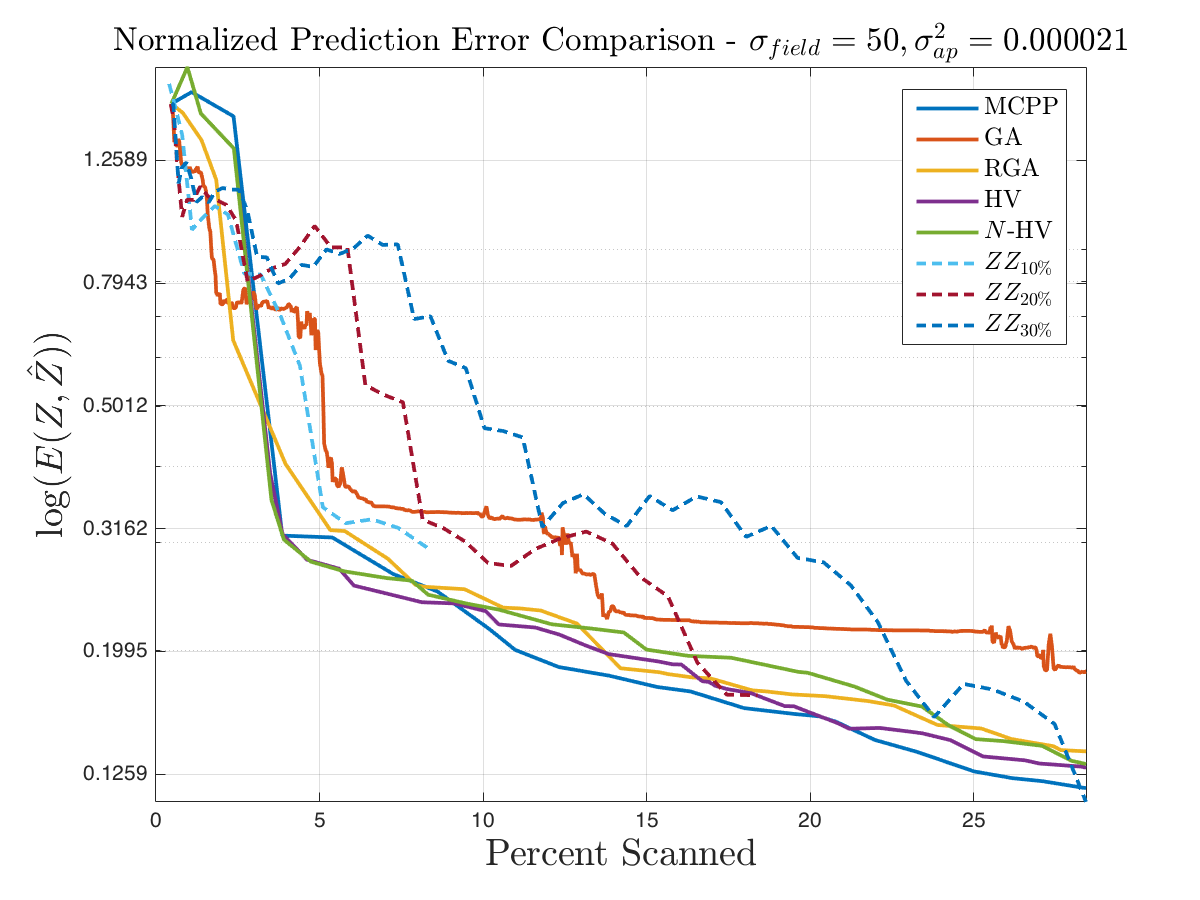
\includegraphics[width=\linewidth]{figures/results/normalized_errors_30p_100x100_sf_50_seed_2_app_50.png}
        \ssp
        \captionsetup{skip=0.20\baselineskip,size=footnotesize}
        \caption{Normalized prediction errors for each method.}
    \end{subfigure}%
    \begin{subfigure}[t]{0.5\textwidth}
        \centering
        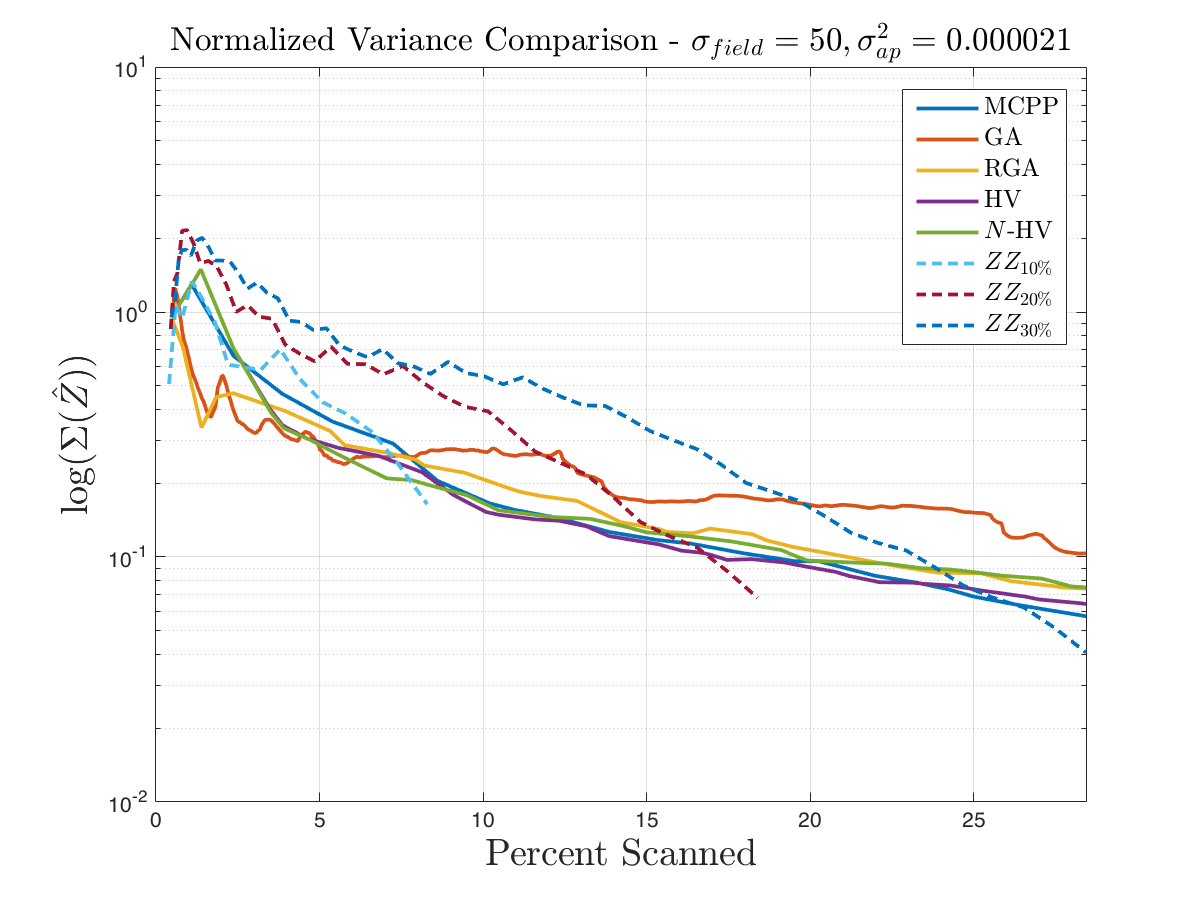
\includegraphics[width=\linewidth]{figures/results/normalized_variances_30p_100x100_sf_50_seed_2_app_50.png}
        \ssp
        \captionsetup{skip=0.20\baselineskip,size=footnotesize}
        \caption{Normalized prediction variances for each method.}
    \end{subfigure}%
    \ssp
    \captionsetup{skip=0.20\baselineskip}
    \caption{Prediction error and variances for an exploration of a field of size $100 \times 100$, $\sigma_{field} = 50$, random seed 2.}
    \label{fig:errvar50}
\end{figure}

\begin{figure}[htb!]
    \centering
        \begin{subfigure}[t]{0.32\textwidth}
        \centering
        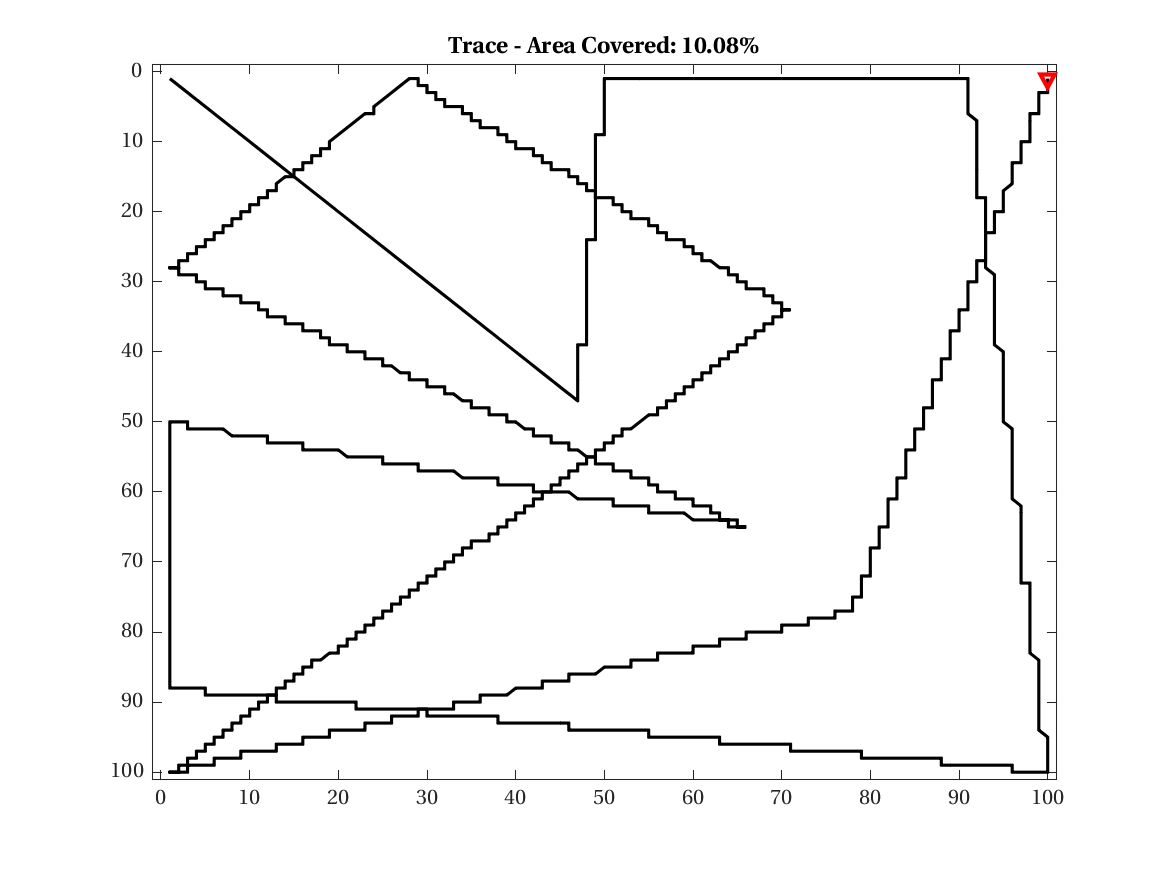
\includegraphics[width=\linewidth]{figures/hbresults/path_nhv_10p_100x100_sf_50_seed_2.png}
        \ssp
        \captionsetup{skip=0.20\baselineskip,size=footnotesize}
        \caption{Highest Variance ($10\%$)}
    \end{subfigure}%
    \begin{subfigure}[t]{0.32\textwidth}
        \centering
        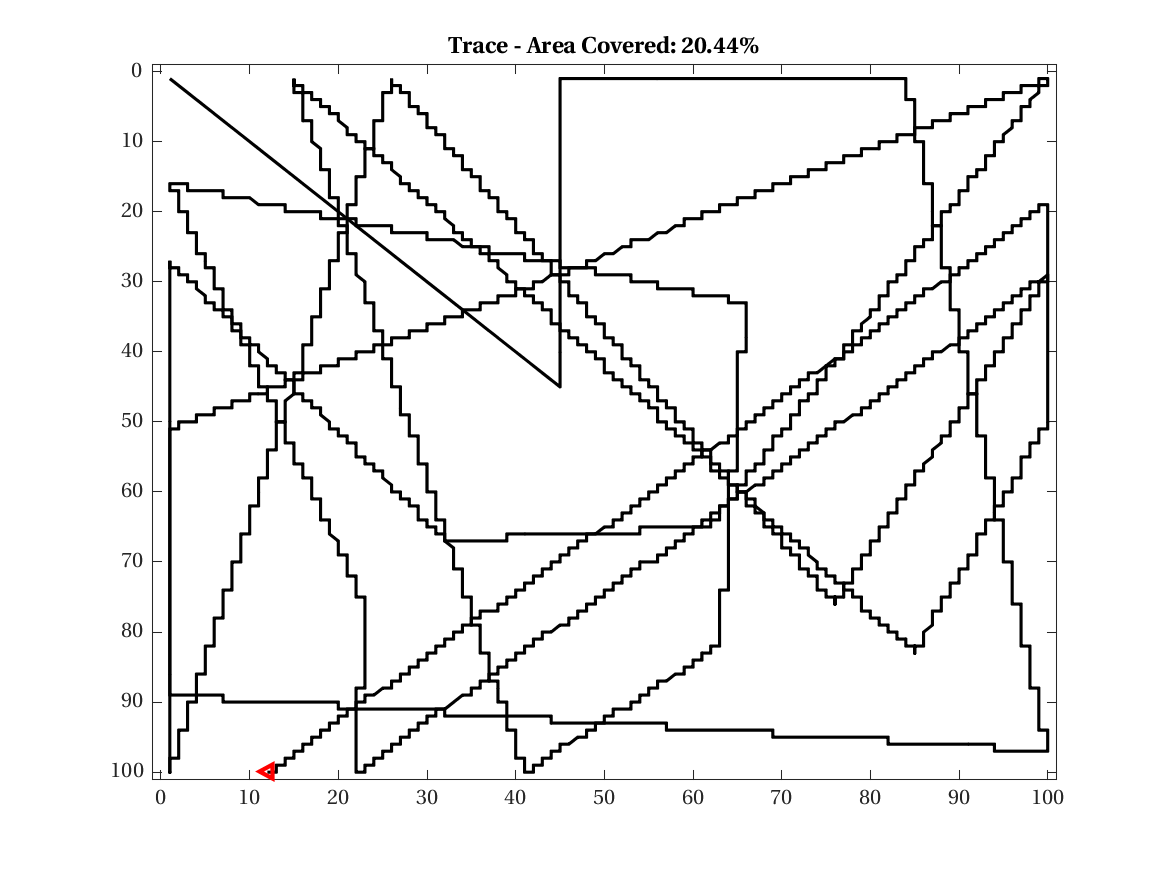
\includegraphics[width=\linewidth]{figures/hbresults/path_nhv_20p_100x100_sf_50_seed_2.png}
        \ssp
        \captionsetup{skip=0.20\baselineskip,size=footnotesize}
        \caption{Highest Variance ($20\%$)}
    \end{subfigure}%
    \begin{subfigure}[t]{0.32\textwidth}
        \centering
        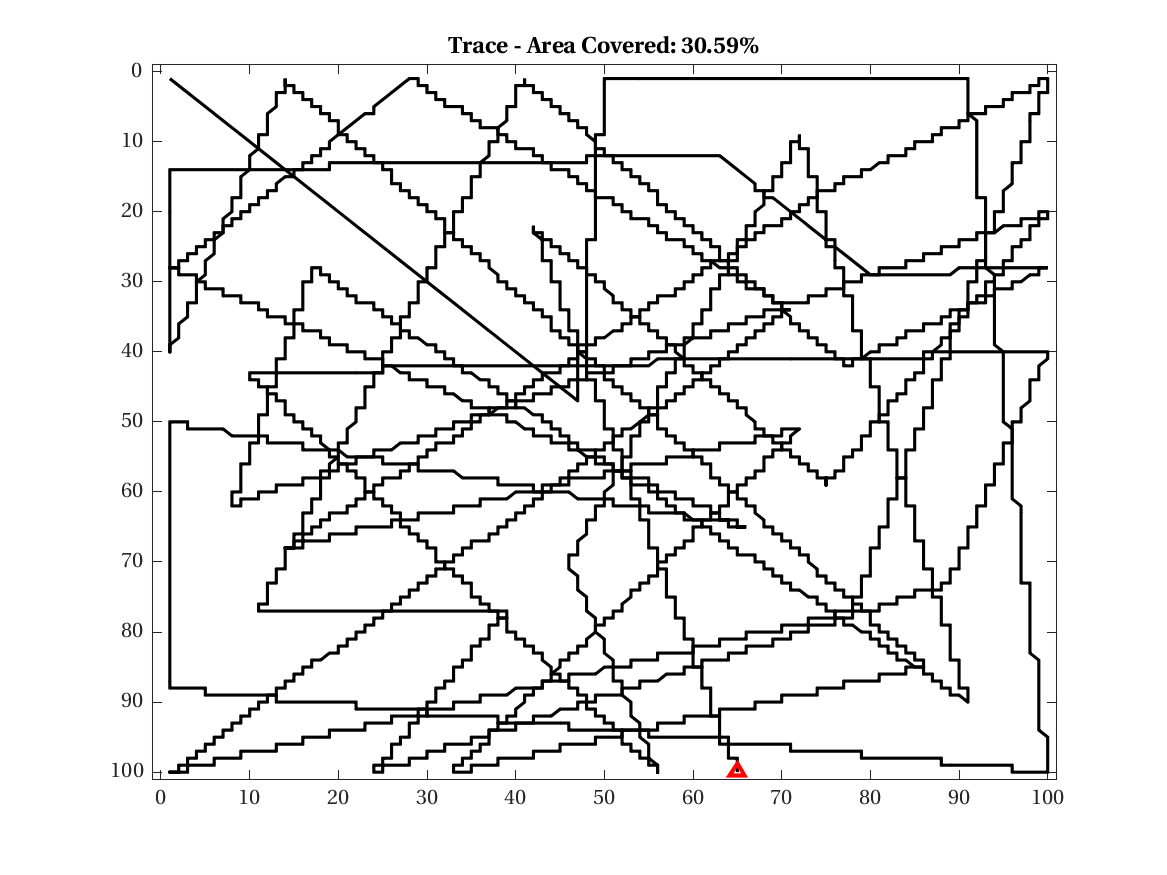
\includegraphics[width=\linewidth]{figures/hbresults/path_nhv_30p_100x100_sf_50_seed_2.png}
        \ssp
        \captionsetup{skip=0.20\baselineskip,size=footnotesize}
        \caption{Highest Variance ($30\%$)}
    \end{subfigure}%
    \\
    \begin{subfigure}[t]{0.32\textwidth}
        \centering
        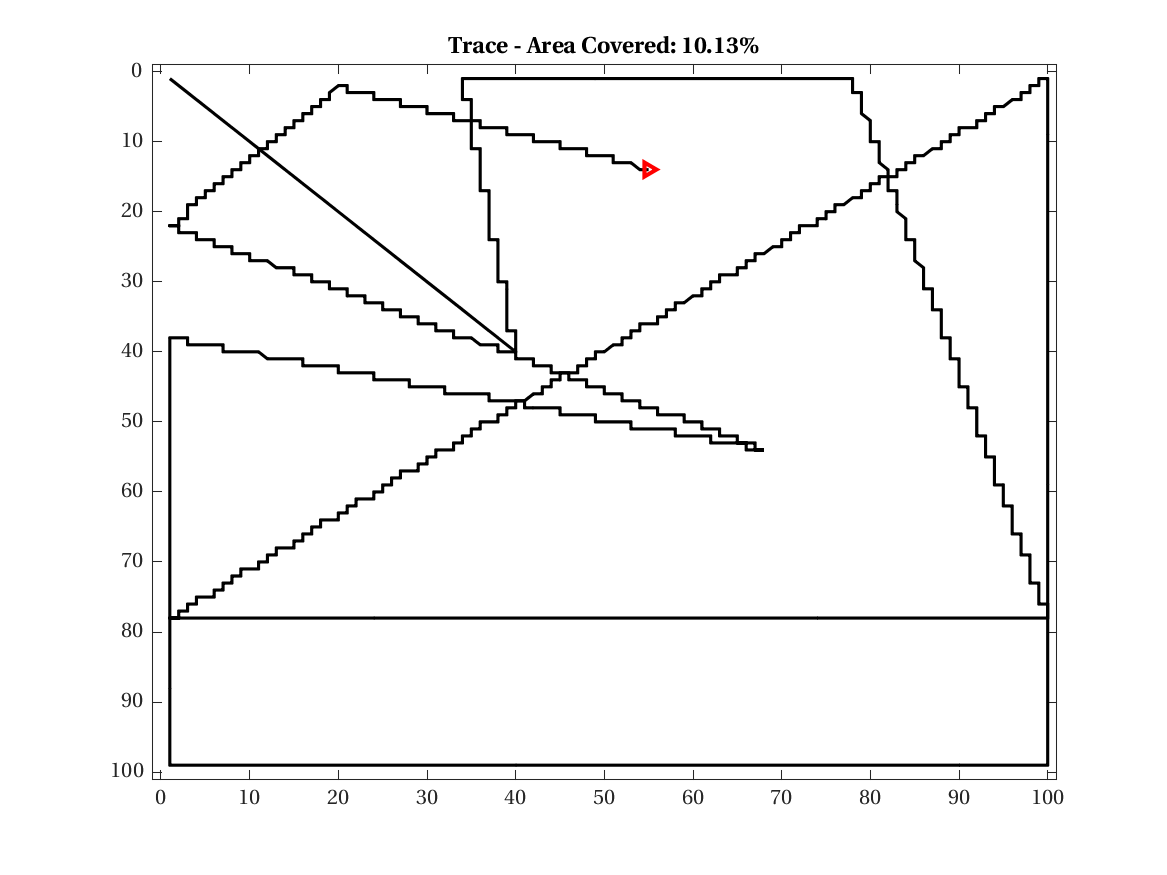
\includegraphics[width=\linewidth]{figures/hbresults/path_nnhv_10p_100x100_sf_50_seed_2.png}
        \ssp
        \captionsetup{skip=0.20\baselineskip,size=footnotesize}
        \caption{$N$ Highest Variance ($10\%$)}
    \end{subfigure}%
    \begin{subfigure}[t]{0.32\textwidth}
        \centering
        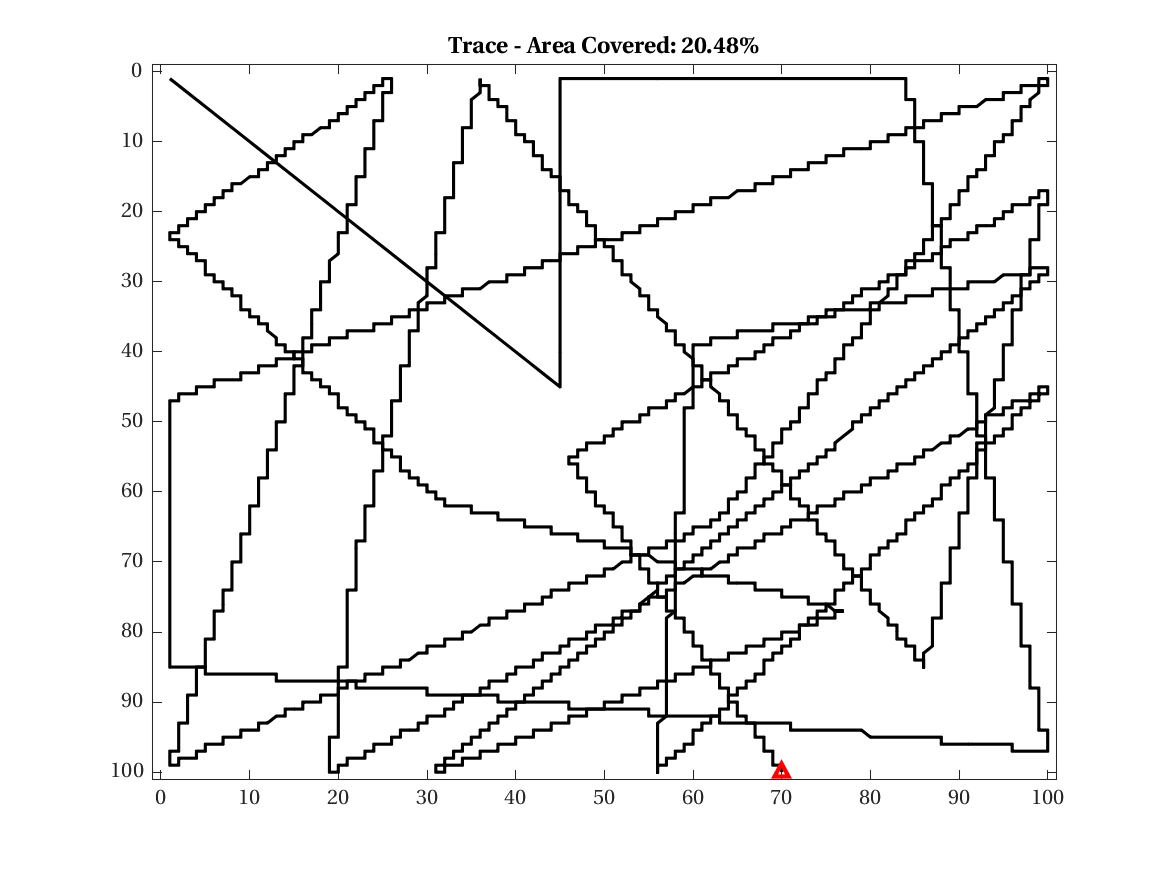
\includegraphics[width=\linewidth]{figures/hbresults/path_nnhv_20p_100x100_sf_50_seed_2.png}
        \ssp
        \captionsetup{skip=0.20\baselineskip,size=footnotesize}
        \caption{$N$ Highest Variance ($20\%$)}
    \end{subfigure}%
    \begin{subfigure}[t]{0.32\textwidth}
        \centering
        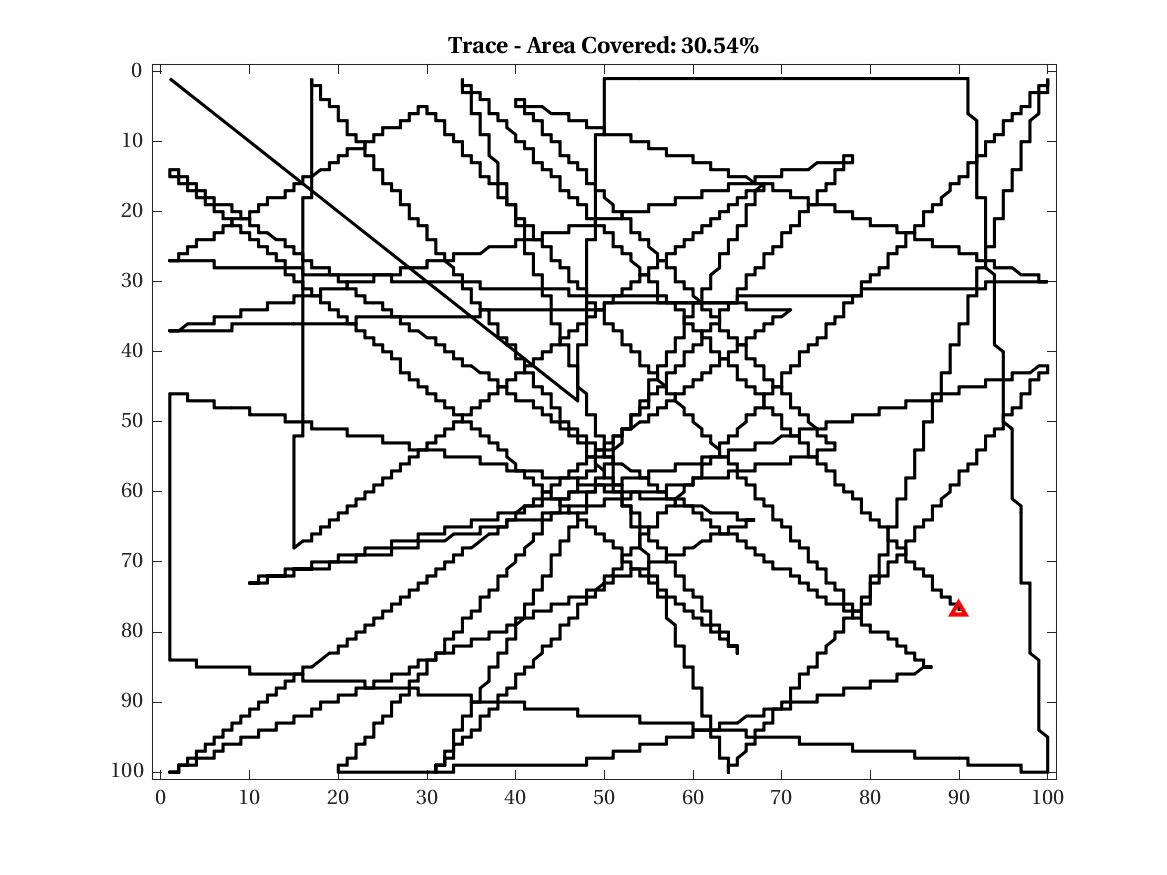
\includegraphics[width=\linewidth]{figures/hbresults/path_nnhv_30p_100x100_sf_50_seed_2.png}
        \ssp
        \captionsetup{skip=0.20\baselineskip,size=footnotesize}
        \caption{$N$ Highest Variance ($30\%$)}
    \end{subfigure}%
    \\
    \begin{subfigure}[t]{0.32\textwidth}
        \centering
        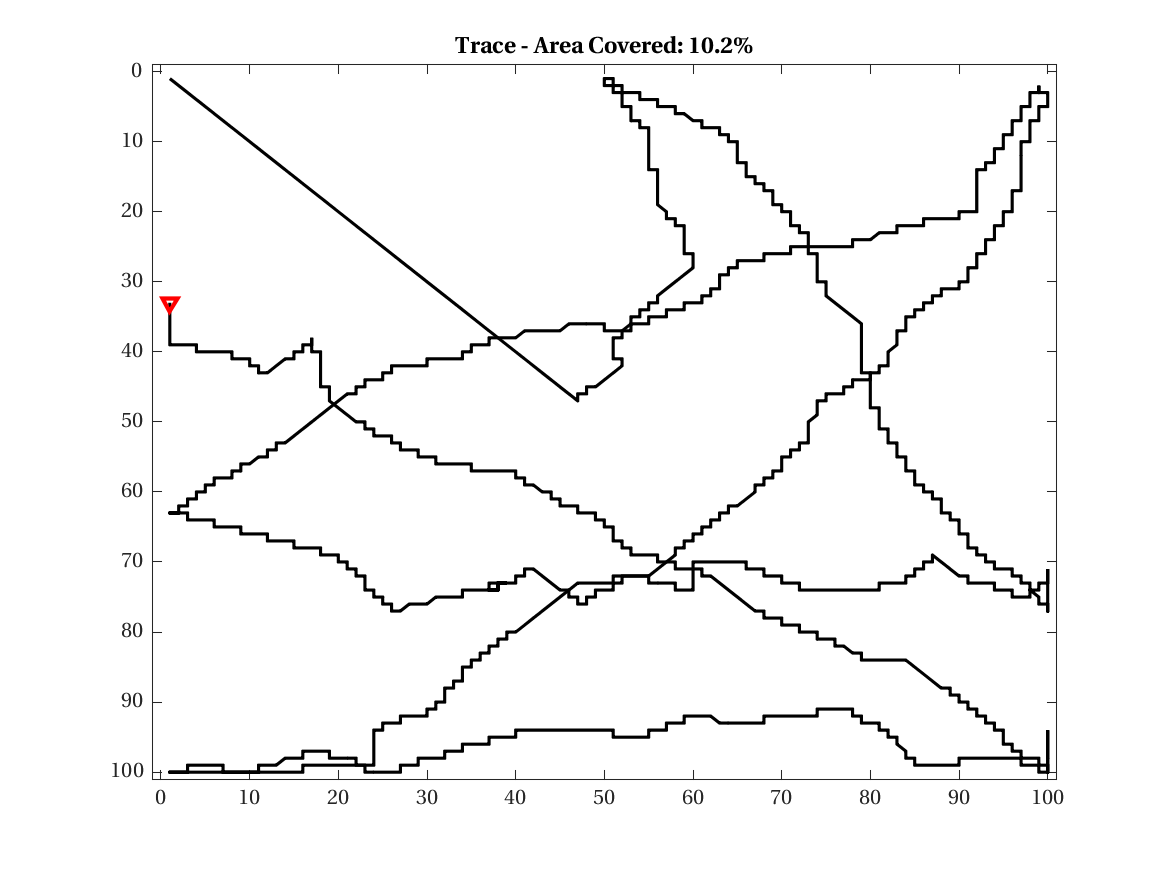
\includegraphics[width=\linewidth]{figures/hbresults/path_mc_10p_100x100_sf_50_seed_2.png}
        \ssp
        \captionsetup{skip=0.20\baselineskip,size=footnotesize}
        \caption{Monte Carlo ($10\%$)}
    \end{subfigure}%
    \begin{subfigure}[t]{0.32\textwidth}
        \centering
        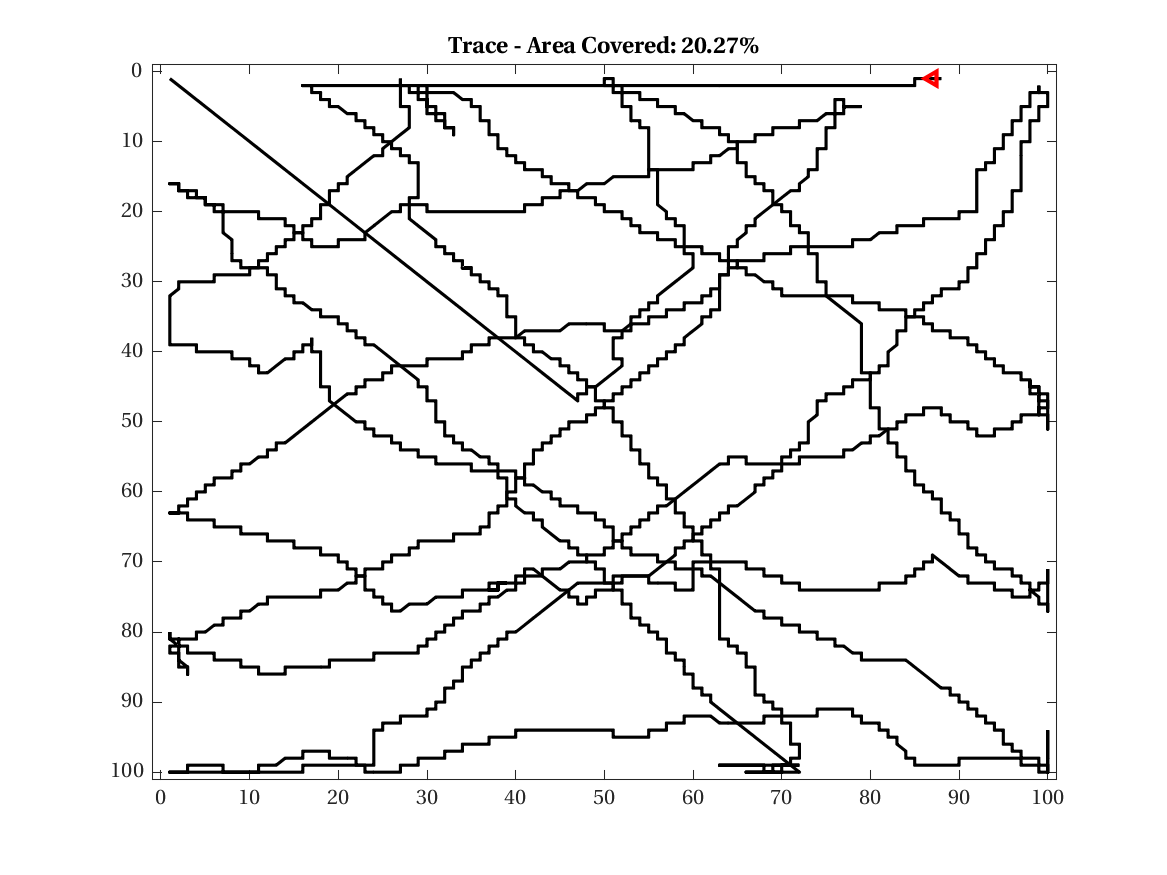
\includegraphics[width=\linewidth]{figures/hbresults/path_mc_20p_100x100_sf_50_seed_2.png}
        \ssp
        \captionsetup{skip=0.20\baselineskip,size=footnotesize}
        \caption{Monte Carlo ($20\%$)}
    \end{subfigure}%
    \begin{subfigure}[t]{0.32\textwidth}
        \centering
        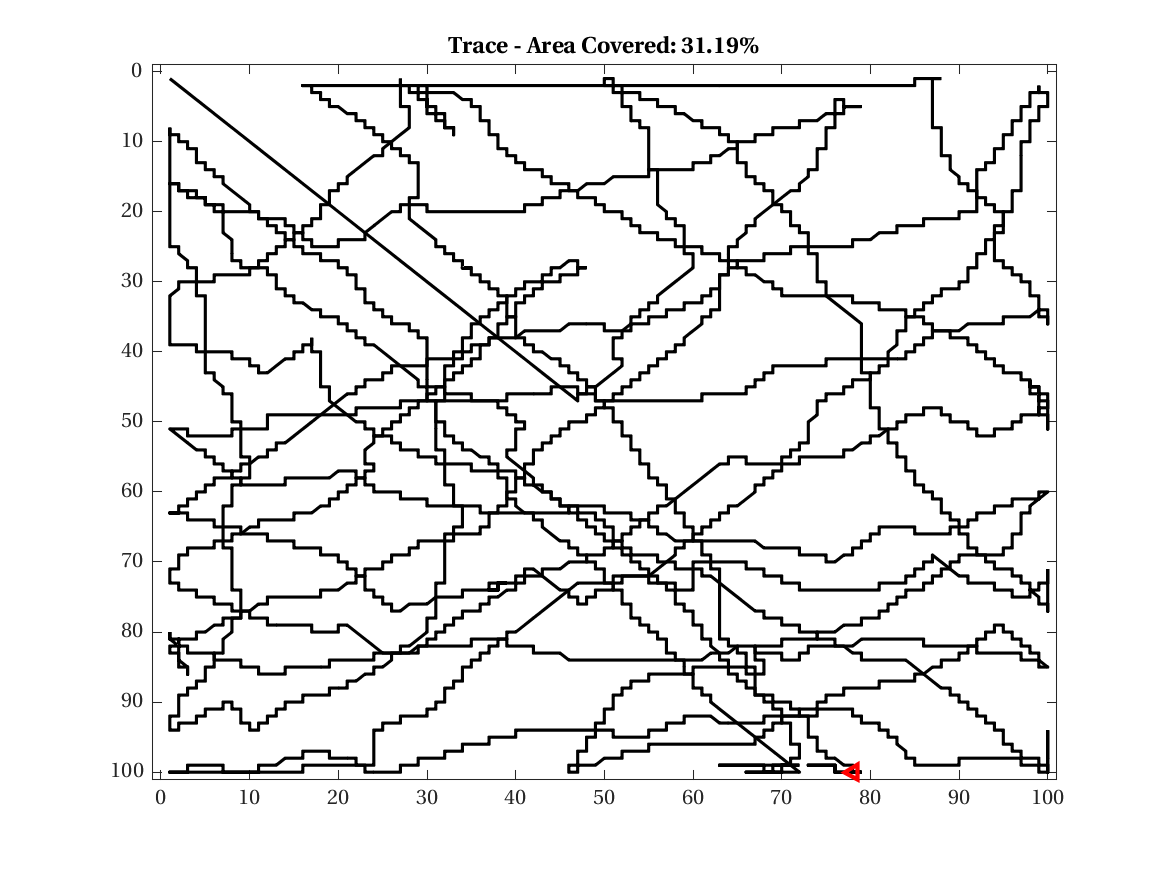
\includegraphics[width=\linewidth]{figures/hbresults/path_mc_30p_100x100_sf_50_seed_2.png}
        \ssp
        \captionsetup{skip=0.20\baselineskip,size=footnotesize}
        \caption{Monte Carlo ($30\%$)}
    \end{subfigure}%
    \\
    \begin{subfigure}[t]{0.32\textwidth}
        \centering
        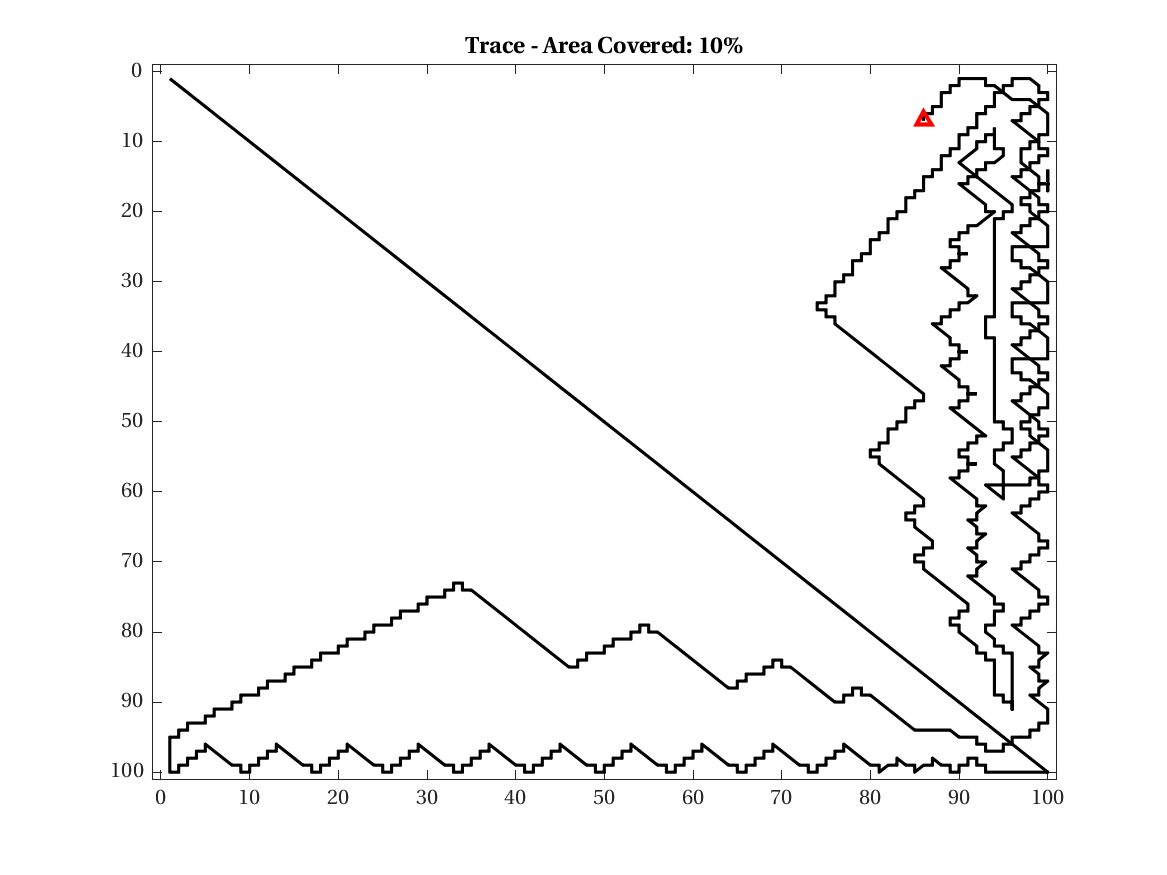
\includegraphics[width=\linewidth]{figures/hbresults/path_gradient_10p_100x100_sf_50_seed_2.png}
        \ssp
        \captionsetup{skip=0.20\baselineskip,size=footnotesize}
        \caption{Gradient Ascent ($10\%$)}
    \end{subfigure}%
    \begin{subfigure}[t]{0.32\textwidth}
        \centering
        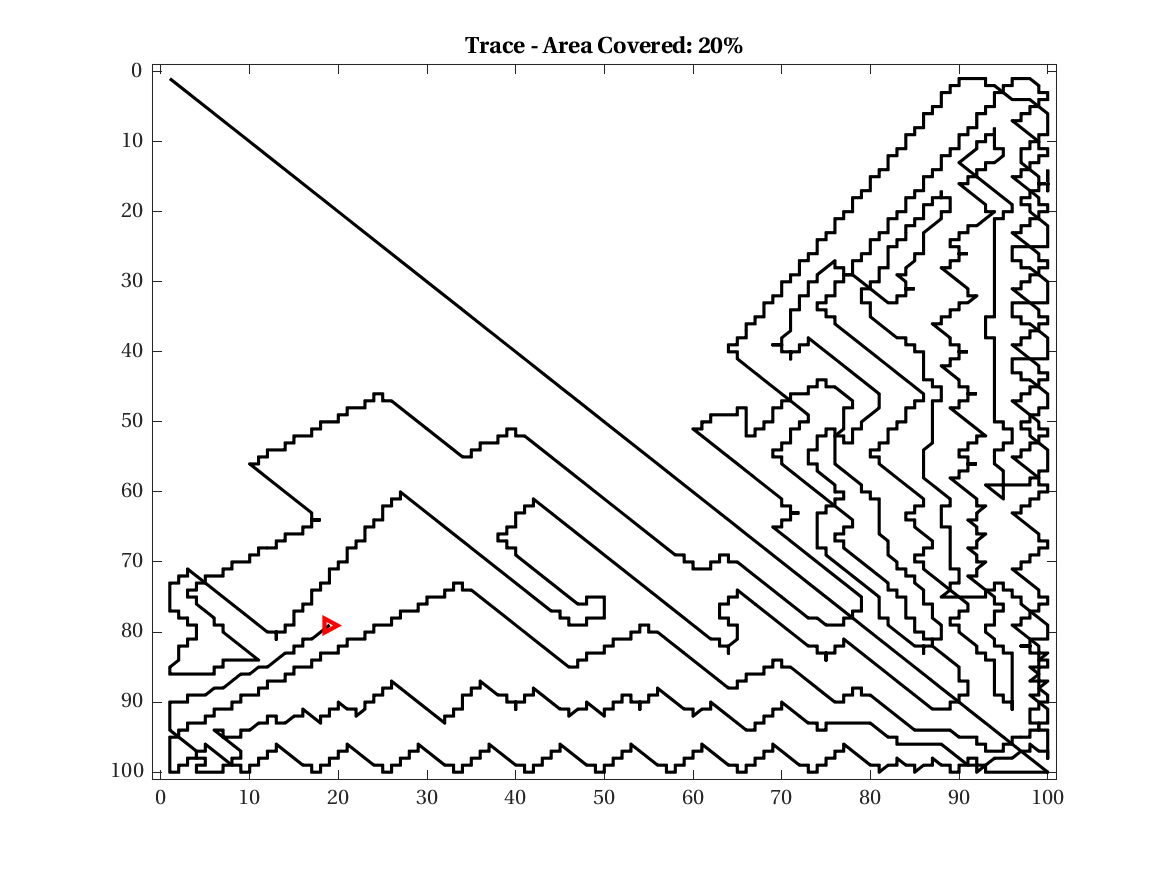
\includegraphics[width=\linewidth]{figures/hbresults/path_gradient_20p_100x100_sf_50_seed_2.png}
        \ssp
        \captionsetup{skip=0.20\baselineskip,size=footnotesize}
        \caption{Gradient Ascent ($20\%$)}
    \end{subfigure}%
    \begin{subfigure}[t]{0.32\textwidth}
        \centering
        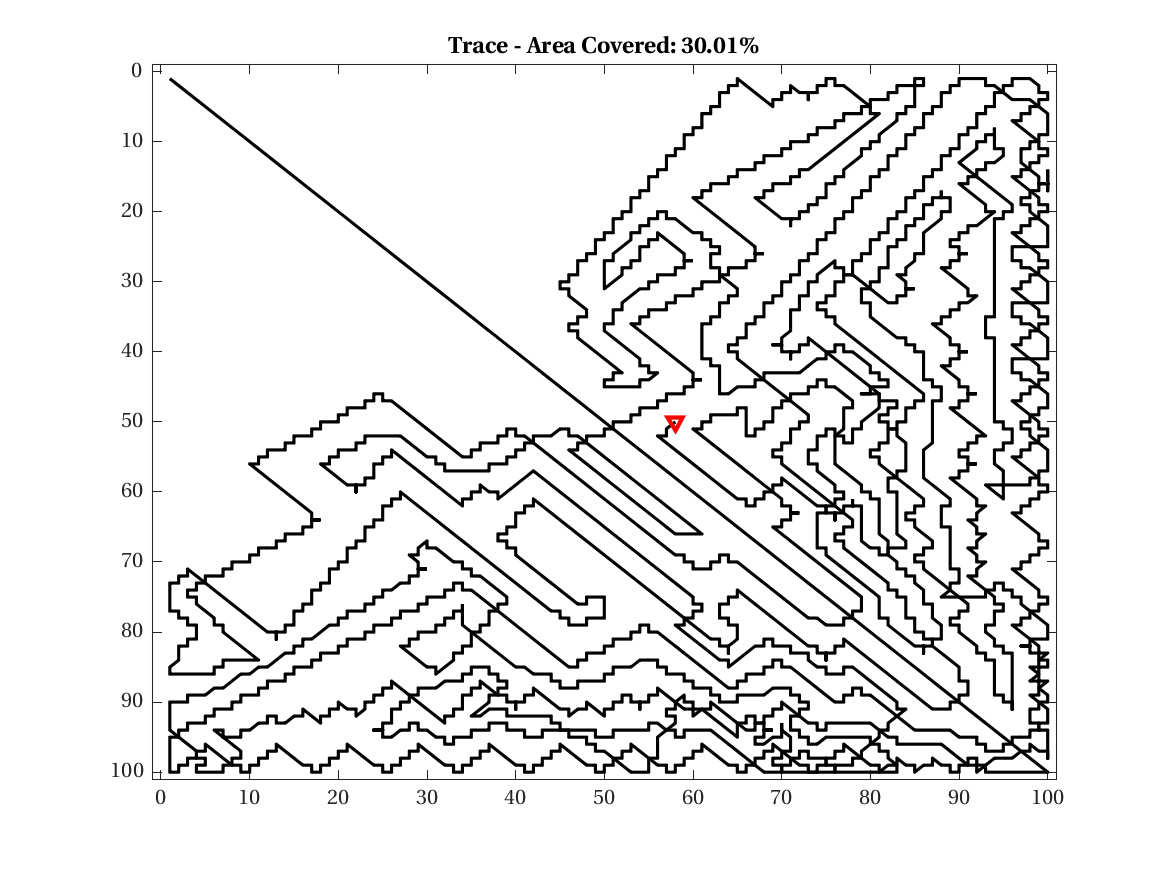
\includegraphics[width=\linewidth]{figures/hbresults/path_gradient_30p_100x100_sf_50_seed_2.png}
        \ssp
        \captionsetup{skip=0.20\baselineskip,size=footnotesize}
        \caption{Gradient Ascent ($30\%$)}
    \end{subfigure}%
    \\
    \begin{subfigure}[t]{0.32\textwidth}
        \centering
        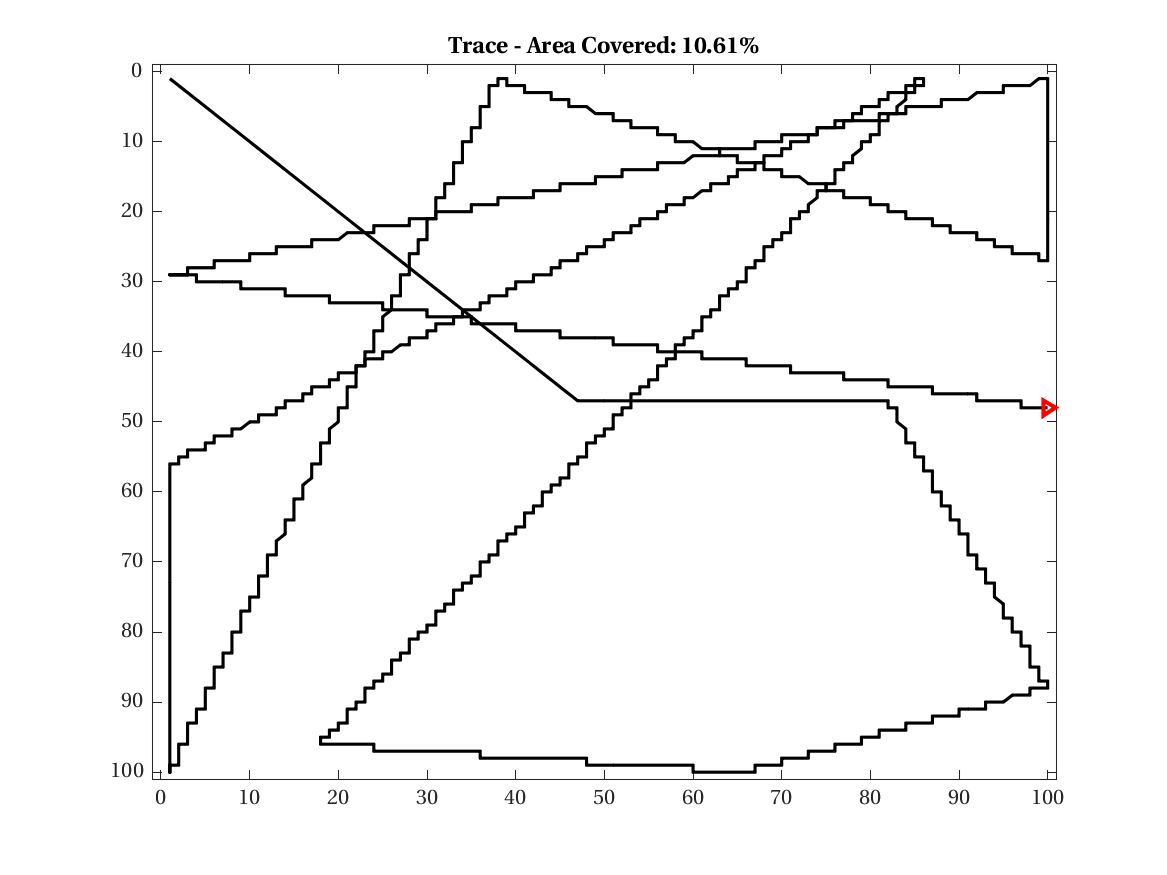
\includegraphics[width=\linewidth]{figures/hbresults/path_gr_10p_100x100_sf_50_seed_2.png}
        \ssp
        \captionsetup{skip=0.20\baselineskip,size=footnotesize}
        \caption{Range Gradient Ascent ($10\%$)}
    \end{subfigure}%
    \begin{subfigure}[t]{0.32\textwidth}
        \centering
        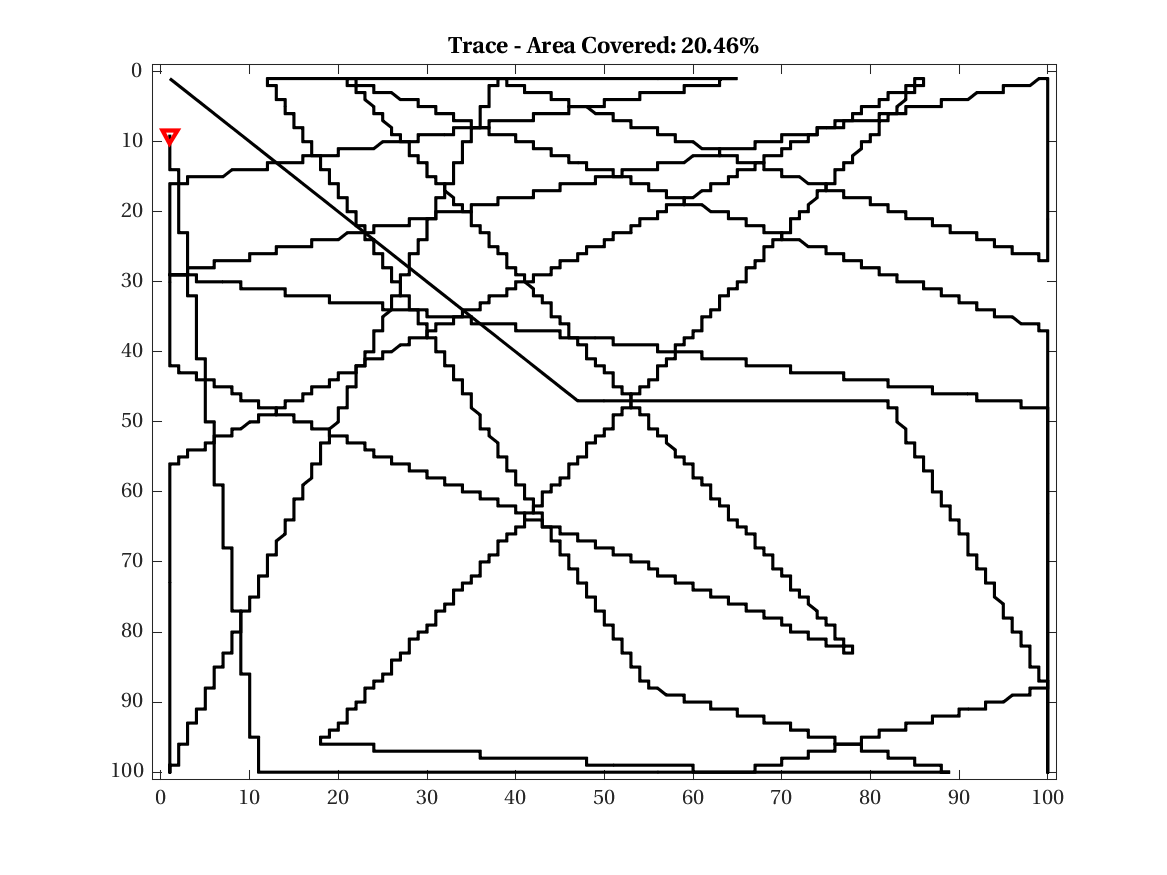
\includegraphics[width=\linewidth]{figures/hbresults/path_gr_20p_100x100_sf_50_seed_2.png}
        \ssp
        \captionsetup{skip=0.20\baselineskip,size=footnotesize}
        \caption{Range Gradient Ascent ($20\%$)}
    \end{subfigure}%
    \begin{subfigure}[t]{0.32\textwidth}
        \centering
        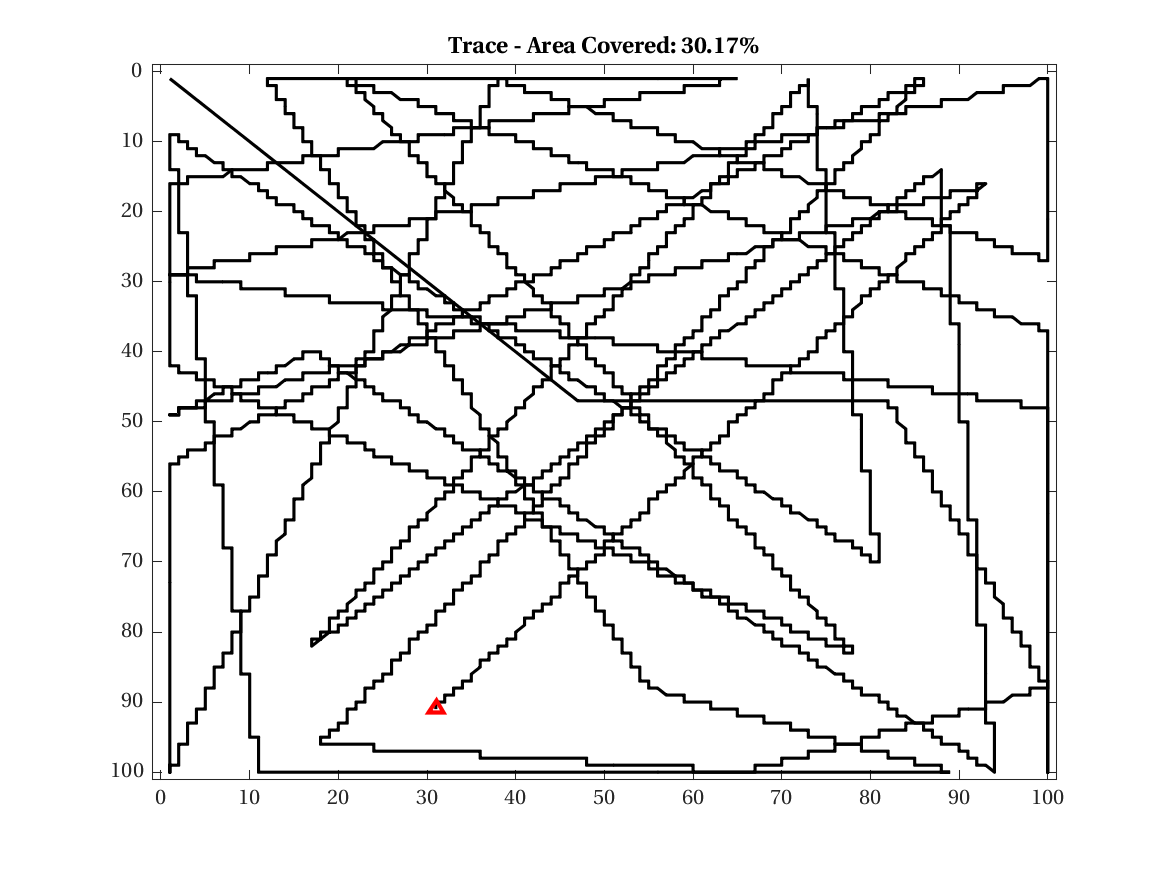
\includegraphics[width=\linewidth]{figures/hbresults/path_gr_30p_100x100_sf_50_seed_2.png}
        \ssp
        \captionsetup{skip=0.20\baselineskip,size=footnotesize}
        \caption{Range Gradient Ascent ($30\%$)}
    \end{subfigure}%
    \ssp
    \captionsetup{skip=0.20\baselineskip}
    \caption{Exploration of a field of size $100 \times 100$, $\sigma_{field} = 50$, random seed 2.}
    \label{fig:sf50}
\end{figure}

\FloatBarrier
\clearpage

\section{Low Spatial Autocorrelation Results ($\sigma_{field} = 1$)} \label{sec:sigma1}

The methods will be compared on target fields generated with an autocorrelation factor, $\sigma_{field}$, equal to one. A Gaussian filter $G(x,y,1)$ (Equation \ref{eq:gauss_filt}), is convolved with all points on the field. Paths taken for each of the methods, except for the zig-zag method, are shown for scan areas nearest to the $10\%$, $20\%$, and $30\%$ marks in Figure \ref{fig:sf1}. \\\\

\begin{figure}[htb!]
    \centering
    \begin{subfigure}[t]{0.5\textwidth}
        \centering
        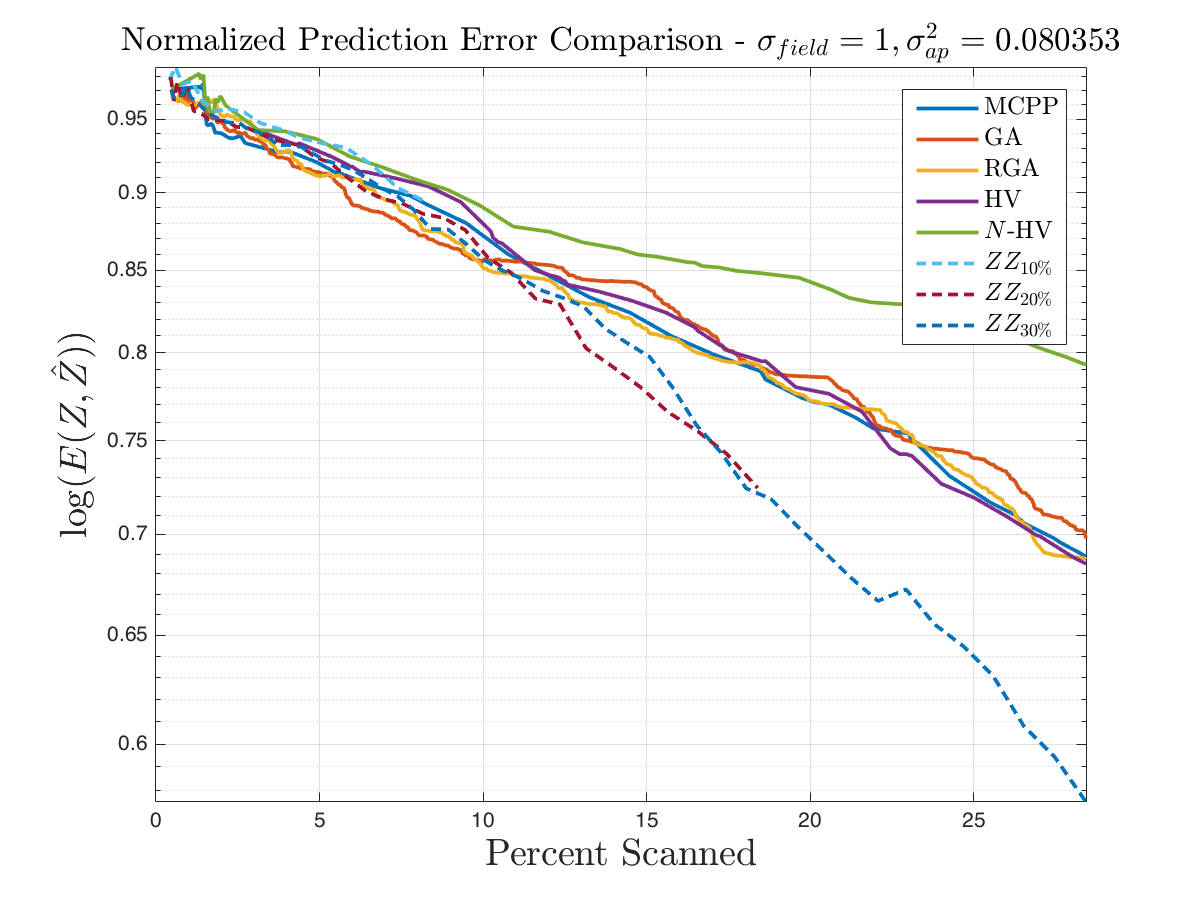
\includegraphics[width=\linewidth]{figures/results/normalized_errors_30p_100x100_sf_1_seed_2_app_50.png}
        \ssp
        \captionsetup{skip=0.20\baselineskip,size=footnotesize}
        \caption{Normalized prediction errors for each method.}
    \end{subfigure}%
    \begin{subfigure}[t]{0.5\textwidth}
        \centering
        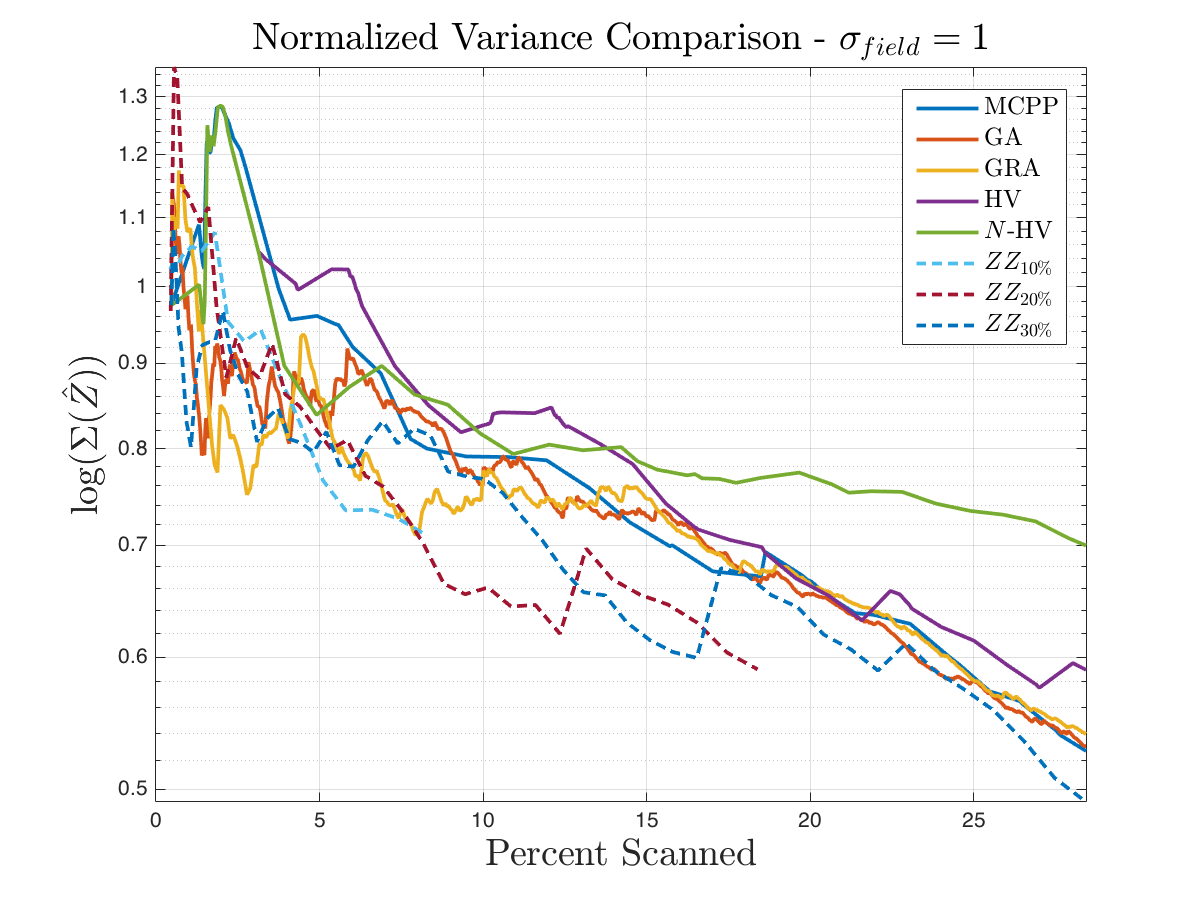
\includegraphics[width=\linewidth]{figures/results/normalized_variances_30p_100x100_sf_1_seed_2_app_50.png}
        \ssp
        \captionsetup{skip=0.20\baselineskip,size=footnotesize}
        \caption{Normalized prediction variances for each method.}
    \end{subfigure}%
    \ssp
    \captionsetup{skip=0.20\baselineskip}
    \caption{Prediction error and variances for an exploration of a field of size $100 \times 100$, $\sigma_{field} = 1$, random seed 2.}
    \label{fig:errvar1}
\end{figure}

\begin{figure}[htb!]
    \centering
        \begin{subfigure}[t]{0.32\textwidth}
        \centering
        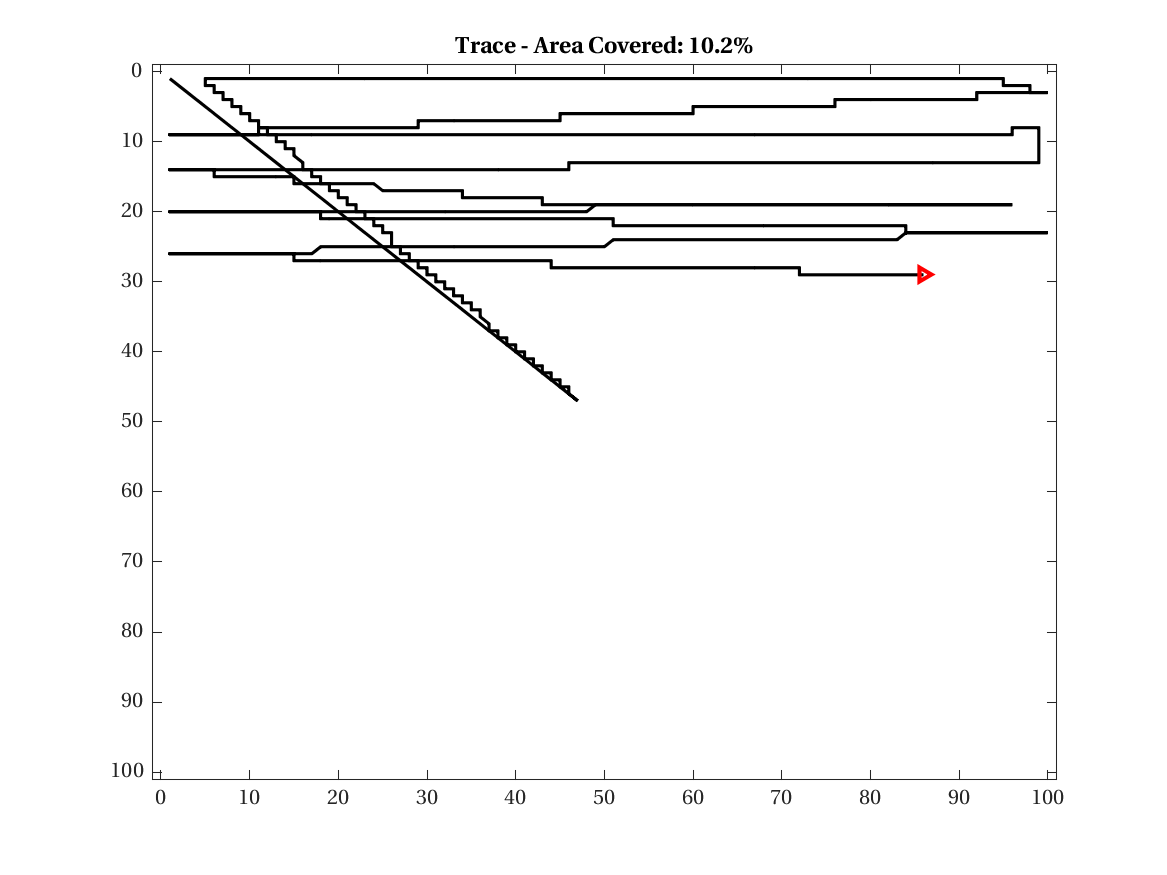
\includegraphics[width=\linewidth]{figures/hbresults/path_nhv_10p_100x100_sf_1_seed_2.png}
        \ssp
        \captionsetup{skip=0.20\baselineskip,size=footnotesize}
        \caption{Highest Variance ($10\%$)}
    \end{subfigure}%
    \begin{subfigure}[t]{0.32\textwidth}
        \centering
        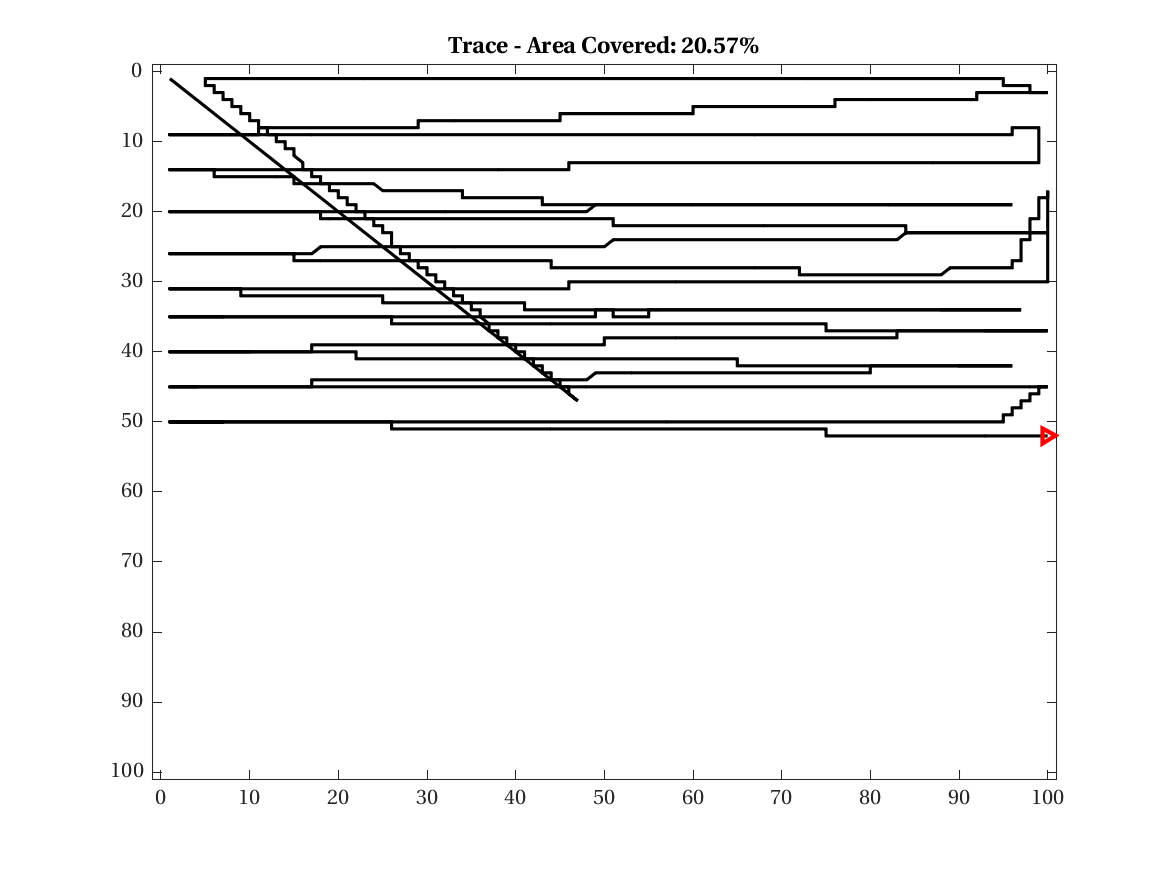
\includegraphics[width=\linewidth]{figures/hbresults/path_nhv_20p_100x100_sf_1_seed_2.png}
        \ssp
        \captionsetup{skip=0.20\baselineskip,size=footnotesize}
        \caption{Highest Variance ($20\%$)}
    \end{subfigure}%
    \begin{subfigure}[t]{0.32\textwidth}
        \centering
        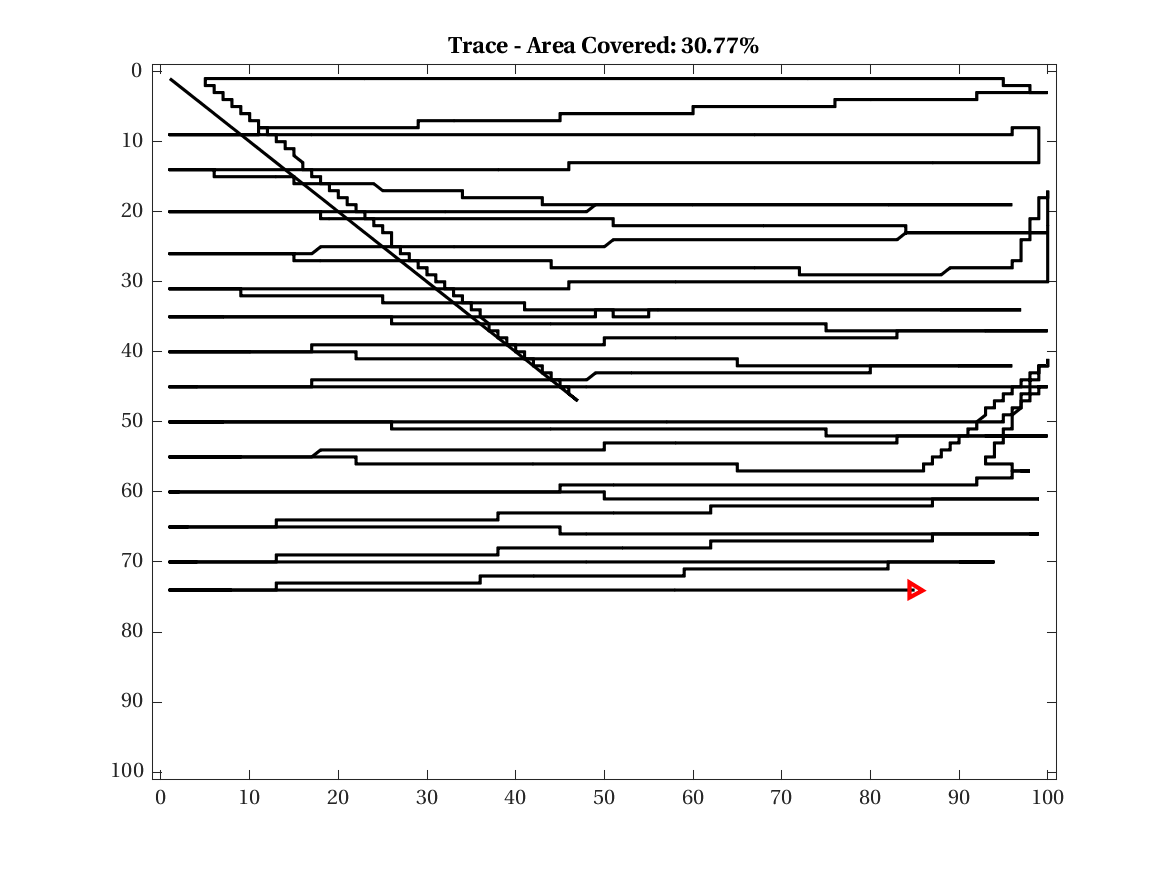
\includegraphics[width=\linewidth]{figures/hbresults/path_nhv_30p_100x100_sf_1_seed_2.png}
        \ssp
        \captionsetup{skip=0.20\baselineskip,size=footnotesize}
        \caption{Highest Variance ($30\%$)}
    \end{subfigure}%
    \\
    \begin{subfigure}[t]{0.32\textwidth}
        \centering
        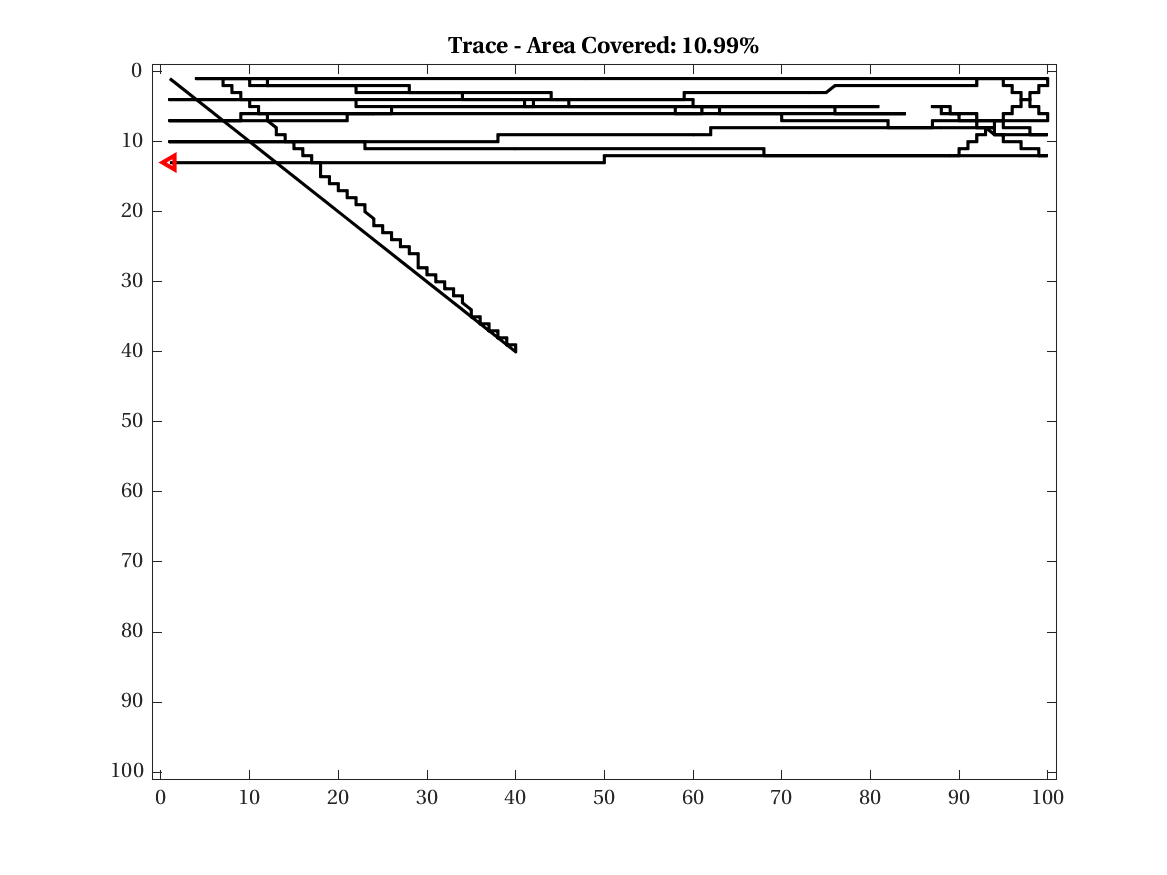
\includegraphics[width=\linewidth]{figures/hbresults/path_nnhv_10p_100x100_sf_1_seed_2.png}
        \ssp
        \captionsetup{skip=0.20\baselineskip,size=footnotesize}
        \caption{$N$ Highest Variance ($10\%$)}
    \end{subfigure}%
    \begin{subfigure}[t]{0.32\textwidth}
        \centering
        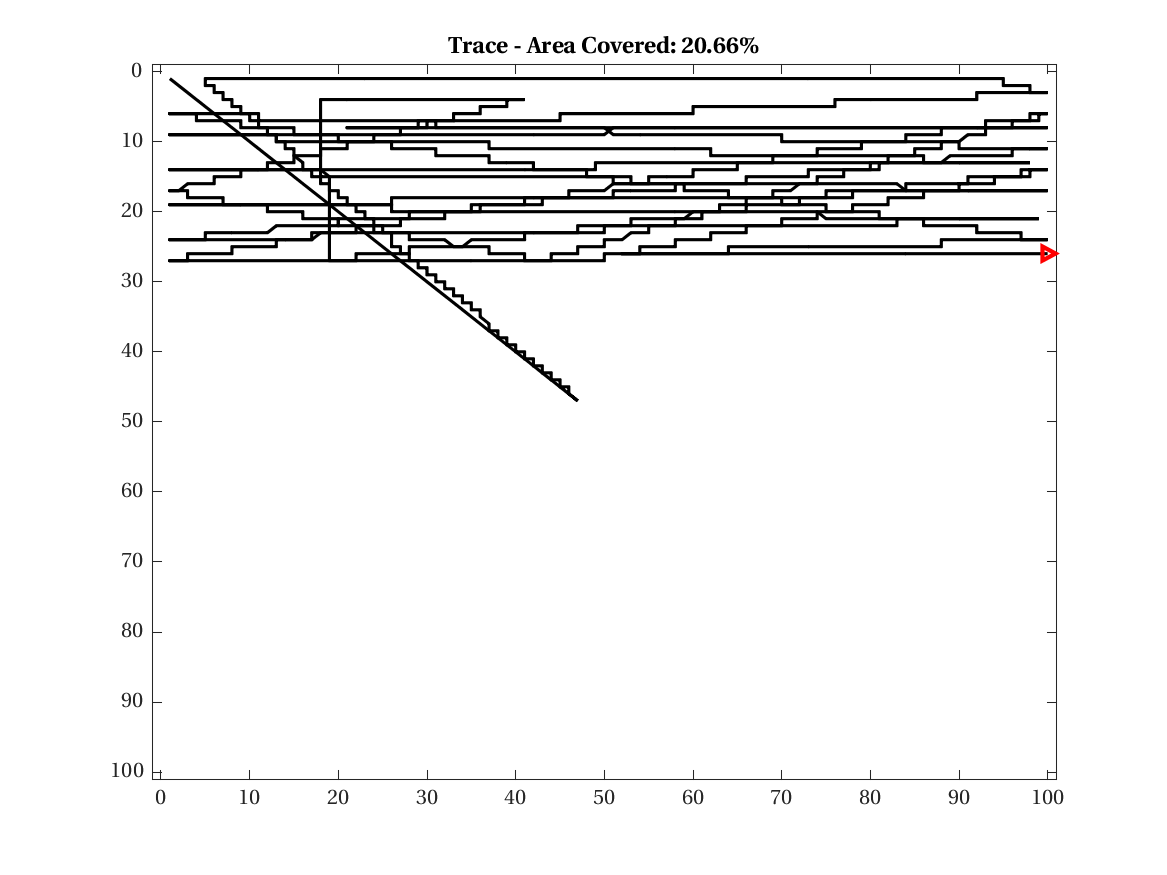
\includegraphics[width=\linewidth]{figures/hbresults/path_nnhv_20p_100x100_sf_1_seed_2.png}
        \ssp
        \captionsetup{skip=0.20\baselineskip,size=footnotesize}
        \caption{$N$ Highest Variance ($20\%$)}
    \end{subfigure}%
    \begin{subfigure}[t]{0.32\textwidth}
        \centering
        \includegraphics[width=\linewidth]{figures/hbresults/path_nnhv_30p_100x100_sf_1_seed_2.png}
        \ssp
        \captionsetup{skip=0.20\baselineskip,size=footnotesize}
        \caption{$N$ Highest Variance ($30\%$)}
    \end{subfigure}%
    \\
    \begin{subfigure}[t]{0.32\textwidth}
        \centering
        \includegraphics[width=\linewidth]{figures/hbresults/path_mc_10p_100x100_sf_1_seed_2.png}
        \ssp
        \captionsetup{skip=0.20\baselineskip,size=footnotesize}
        \caption{Monte Carlo ($10\%$)}
    \end{subfigure}%
    \begin{subfigure}[t]{0.32\textwidth}
        \centering
        \includegraphics[width=\linewidth]{figures/hbresults/path_mc_20p_100x100_sf_1_seed_2.png}
        \ssp
        \captionsetup{skip=0.20\baselineskip,size=footnotesize}
        \caption{Monte Carlo ($20\%$)}
    \end{subfigure}%
    \begin{subfigure}[t]{0.32\textwidth}
        \centering
        \includegraphics[width=\linewidth]{figures/hbresults/path_mc_30p_100x100_sf_1_seed_2.png}
        \ssp
        \captionsetup{skip=0.20\baselineskip,size=footnotesize}
        \caption{Monte Carlo ($30\%$)}
    \end{subfigure}%
    \\
    \begin{subfigure}[t]{0.32\textwidth}
        \centering
        \includegraphics[width=\linewidth]{figures/hbresults/path_gradient_10p_100x100_sf_1_seed_2.png}
        \ssp
        \captionsetup{skip=0.20\baselineskip,size=footnotesize}
        \caption{Gradient Ascent ($10\%$)}
    \end{subfigure}%
    \begin{subfigure}[t]{0.32\textwidth}
        \centering
        \includegraphics[width=\linewidth]{figures/hbresults/path_gradient_20p_100x100_sf_1_seed_2.png}
        \ssp
        \captionsetup{skip=0.20\baselineskip,size=footnotesize}
        \caption{Gradient Ascent ($20\%$)}
    \end{subfigure}%
    \begin{subfigure}[t]{0.32\textwidth}
        \centering
        \includegraphics[width=\linewidth]{figures/hbresults/path_gradient_30p_100x100_sf_1_seed_2.png}
        \ssp
        \captionsetup{skip=0.20\baselineskip,size=footnotesize}
        \caption{Gradient Ascent ($30\%$)}
    \end{subfigure}%
    \\
    \begin{subfigure}[t]{0.32\textwidth}
        \centering
        \includegraphics[width=\linewidth]{figures/hbresults/path_gr_10p_100x100_sf_1_seed_2.png}
        \ssp
        \captionsetup{skip=0.20\baselineskip,size=footnotesize}
        \caption{Range Gradient Ascent ($10\%$)}
    \end{subfigure}%
    \begin{subfigure}[t]{0.32\textwidth}
        \centering
        \includegraphics[width=\linewidth]{figures/hbresults/path_gr_20p_100x100_sf_1_seed_2.png}
        \ssp
        \captionsetup{skip=0.20\baselineskip,size=footnotesize}
        \caption{Range Gradient Ascent ($20\%$)}
    \end{subfigure}%
    \begin{subfigure}[t]{0.32\textwidth}
        \centering
        \includegraphics[width=\linewidth]{figures/hbresults/path_gr_30p_100x100_sf_1_seed_2.png}
        \ssp
        \captionsetup{skip=0.20\baselineskip,size=footnotesize}
        \caption{Range Gradient Ascent ($30\%$)}
    \end{subfigure}%
    \ssp
    \captionsetup{skip=0.20\baselineskip}
    \caption{Exploration of a field of size $100 \times 100$, $\sigma_{field} = 1$, random seed 2.}
    \label{fig:sf1}
\end{figure}

\FloatBarrier
\clearpage